\documentclass{article}

\usepackage{amsmath, amsthm, amssymb, amsfonts}
\usepackage{thmtools}
\usepackage{graphicx}
\usepackage{setspace}
\usepackage{geometry}
\usepackage{float}
\usepackage{hyperref}
\usepackage[utf8]{inputenc}
\usepackage[english]{babel}
\usepackage{framed}
\usepackage[dvipsnames]{xcolor}
\usepackage{tcolorbox}
\usepackage{tikz}
\usetikzlibrary{patterns}
\colorlet{LightGray}{White!90!Periwinkle}
\colorlet{LightOrange}{Orange!15}
\colorlet{LightGreen}{Green!15}

\newcommand{\HRule}[1]{\rule{\linewidth}{#1}}

\declaretheoremstyle[name=,]{thmsty}
\declaretheorem[style=thmsty,numberwithin=section]{theorem}
\tcolorboxenvironment{theorem}{colback=LightGray}

\declaretheoremstyle[name=Proposition,]{prosty}
\declaretheorem[style=prosty,numberlike=theorem]{proposition}
\tcolorboxenvironment{proposition}{colback=LightOrange}

\declaretheoremstyle[name=Principle,]{prcpsty}
\declaretheorem[style=prcpsty,numberlike=theorem]{principle}
\tcolorboxenvironment{principle}{colback=LightGreen}

\setstretch{1.2}
\geometry{
    textheight=9in,
    textwidth=5.5in,
    top=1in,
    headheight=12pt,
    headsep=25pt,
    footskip=30pt
}

% ------------------------------------------------------------------------------

\begin{document}

% ------------------------------------------------------------------------------
% Cover Page and ToC
% ------------------------------------------------------------------------------

\title{ \normalsize \textsc{Topology and Differential Geometry}
		\\ [2.0cm]
		\HRule{1.5pt} \\
        \LARGE \textbf{\uppercase{A lecture note on Topology and Differential Geometry for Noob Wannabe Physicists}
		\HRule{2.0pt} \\ [0.6cm] \LARGE{} \vspace*{10\baselineskip}}
		}
        %\date{}
\author{\textbf{Author} \\ 
		Mushrafi Munim Sushmit \\
		Department of Physics, University of Dhaka \\
		}

\maketitle
\newpage

\tableofcontents
\newpage

\section*{Preface} % The asterisk prevents LaTeX from numbering the section
\addcontentsline{toc}{section}{Preface} 

This document draws primarily from the online lectures delivered by Professor Sunil Mukhi, which are available on YouTube. Many of the definitions, proofs, and certain sections are directly sourced from his book, Lectures on Advanced Mathematical Methods for Physicists. For more rigorous proofs go through Lecture Notes on Elementary Topology and Geometry by Itzhak Singer and John Thorpe.

\newpage 


% ------------------------------------------------------------------------------

\section{Topology}

Let's start with basic function definitions. 

\textbf{Surjective :} There is always an $ a \in A $ such that $ \forall b \in B $ there is a functional mapping from $ A :\rightarrow B $ \\ 
\textbf{Injective :} $ \forall a \in A $ and $ \forall b \in B $ there is an one to one functional mapping $ A :\rightarrow B $ \\ 
\textbf{Bijective :} When both Surjective and Injective work. that means $
\forall a \in A, \forall b \in B
$ we have $ f(a) = b $

\subsection{Topological Space}
The motivation is to capture the concept of continuity without assuming calculus. This is an 19th century development. Physicists want to capture a more general structure without using calculus such that this new thing can be used in both calculus and some other stuffs. 

We should first shed off the idea of Vector spaces or other mathematical structure. It will be helpful to consider the whole idea of Topological space as an abstract space that can accomodate any mathematical spaces. 

To start off our journey, let's try to define the limit we studied in calculus in Topology.We will try to generalize the concept of limit and continuity such that it can be used in a more generalize fashion. 

\begin{theorem}
  An open set is defined as $ x \in X \rightarrow x \in (a,b) \subset X $
\end{theorem}

What it means is that if we take any elements from $ X $ it will always be smaller than a fixed boundary or greater than a fixed boundary. Another way to look at it is the limits. If we consider an open set in the interval $ x \in (a,b) $ or maybe an infinite set $ x \in (a,\infty) $ then we can always choose a point $ x  $ such that $ | x-a|< \epsilon $
and $ |b-x| < \epsilon $ is always satisfied. \textbf{All points in that set should have the value such that they can be enclosed by an open interval (a,b) }

\begin{theorem}
    A closed set is the compliment of open set.     
\end{theorem}

To prove that the $ x \in [a,b] \subseteq A $ is an element of closed set we take the compliment of $ A $ and we will get $ x \in (\infty, a) \cup  x \in (b,\infty) $. Clearly the latter is an open set so by definition, $ A $, as it is the compliment of an open set, must therefore be a closed set.   

Examples of open set include empty set, Real numbers set, any number line extended to infinity.

Examples of closed set are single points, closed intervals. Even the real numbers and empty sets are also closed sets. They are kind of both open and closed due to the definition. 

A set can be open, closed, both or neither. So it's better not to hung up on this notion. Just treat it as it is. Another thing to keep in mind is that we are dealing with sets not just fixed intervals. 

Now if we combine all of this the formal definition of Topology is thus 

\begin{theorem}
    Let S be an non-empty set and U be a collection of subset of X satisfying the following three conditions 
    \begin{enumerate}
        \item $ \phi \in U, S \in U $ 
        \item For any two subsets $ S_1 \in U $ \& $ S_2 \in U $, then $ S_1 \cap S_2 \subset U $ 
        \item For any two subsets For any two subsets $ S_1 \in U $ \& $ S_2 \in U $, then $ S_1 \cup S_2 \subset U $ 
    \end{enumerate} 
    Then $ (S,U) $ is called the Topological space and the collection $ U $ is called the Topology on $ S $ 
\end{theorem}

We are free to choose the Topology $ U $, we can choose whatever set we want as long as the above conditions are satisfied. 

\begin{proposition}
    Let $ X = {a,b,c} $ and $ T = \{ \phi, X, \{a\}, \{b\}, \{a,b\} \} $ then T is a Topology. but if we had $ T = \{ \phi, X, \{a\}, \{b\}, \{a,b\} , \{c\} \} $, Then this is not a topology. 
    Cause the union of $ \{b\} \cup \{c\} = \{b,c\} \notin T $ 
\end{proposition}

Some definitions 

\begin{itemize}
    \item \textbf{Indiscreet Topology :} When the Topology of Topological space $(S,U)$ involves only the empty set $\phi$ and $S$ 
    \item \textbf{Discreet Topology :} When the topology involves all the subsets possible 
        (power set) 
\end{itemize}

\subsection{Metric Space}
A \textbf{metric space} is a set $M$ together with a function $d: M \times M \to \mathbb{R}^{+}$, called a $\emph{metric}$ or $\emph{distance function}$, such that for all $x, y, z \in M$, the following conditions are satisfied:
\begin{enumerate}
    \item \textbf{Non-negativity:} $d(x, y) \geq 0$.
    \item \textbf{Identity of indiscernibles:} $d(x, y) = 0$ if and only if $x = y$.
    \item \textbf{Symmetry:} $d(x, y) = d(y, x)$.
    \item \textbf{Triangle inequality:} $d(x, z) \leq d(x, y) + d(y, z)$.
\end{enumerate}

It is basically a measuring device. We are all too much engrossed with the cartesian distance formula, which is not necessarily the only formula or the correct formula to measure distance in a higher plane or in a different coordinate system. The above abstract definition allows for a more general set of formulas and is useful. Minkowski space is not a metric space as it violates the above conditions. 

An example of metric space is, on $\mathbb{R}$, we may choose the usual metric $d(x, y) = |x - y|$.     


Now why did we mention this space. Metric space can be used to define a topology. 

\section*{Metric Topology}

Let's start with a \textbf{metric space}. A metric space consists of a set $X$ along with a function $d: X \times X \to \mathbb{R}$, called a \emph{metric}, which measures the distance between any two points in $X$. The \textbf{metric topology} is a way of defining which subsets of $X$ can be called "open". An open set in this context is a set where, for any point within it, you can find a small "neighborhood" around that point which is entirely contained within the set. 

Formally, 

\begin{theorem} 
Let $(X, d)$ be a metric space where $X$ is a set and $d: X \times X \to \mathbb{R}$ is a metric. The \textbf{metric topology} on $X$ is the topology $\mathcal{T}$ generated by the open sets defined using the metric $d$. A subset $U \subseteq X$ is said to be \emph{open} in the metric topology if, for every point $x \in U$, there exists an $\epsilon > 0$ such that the open ball $B_d(x, \epsilon) \subset U$. Here, the open disc $B_d(x, \epsilon)$ is defined as
\[
B_d(x, \epsilon) = \{ y \in X \mid d(x, y) < \epsilon \}.
\]

\end{theorem}

To think of an open disc consider the points enclosed by a circle, but now the boundaries are not inlcuded, means they have an open interval. But it is abstract and defined by the metric. 

The metric topology defines a structure on $X$ that allows us to talk about concepts like continuity, convergence, and compactness in a rigorous way. It turns our set $X$ into a \emph{topological space}, which means it satisfies three key properties:
\begin{enumerate}
    \item The set $X$ itself and the empty set $\emptyset$ are considered open.
    \item Any union of open sets is also open.
    \item Any finite intersection of open sets is also open.
\end{enumerate} 

Examples are given below:
\begin{enumerate}
    \item In the real numbers $\mathbb{R}$, we can define the distance between any two points $x$ and $y$ as $d(x, y) = |x - y|$. The open sets in this metric topology are unions of open intervals, like $(a, b)$, where $a < b$.

    \item In the plane $\mathbb{R}^2$, we define the distance between points $(x_1, y_1)$ and $(x_2, y_2)$ as
    \[
    d((x_1, y_1), (x_2, y_2)) = \sqrt{(x_1 - x_2)^2 + (y_1 - y_2)^2}.
    \]
    The open sets in this metric topology are unions of open disks (circles without the boundary).
\end{enumerate}

It's convenient to use a matric space to define a topology but not the necessity.

\subsection{Topology Basis} 

To understand the concept of a topology, we need to introduce the idea of a \textbf{basis}. A basis helps us define a topology in a more manageable way by specifying a set of "building blocks" for the open sets.

The open intervals on \(\mathbb{R}\) have the following properties:
\begin{itemize}
    \item[(i)] The union of all open intervals is the whole set \(\mathbb{R}\):
    \[
    \bigcup (a_i, b_i) = \mathbb{R}
    \]
    \item[(ii)] The intersection of two open intervals can be expressed as the union of other open intervals. For example, if \(a_1 < a_2 < b_1 < b_2\), then
    \[
    (a_1, b_1) \cap (a_2, b_2) = \bigcup (a_2, b_1)
    \]
    \item[(iii)] \(\emptyset\) is an open interval: \((a, a) = \emptyset\).
\end{itemize}
These properties can be abstracted to define a basis for an arbitrary topological space. 

\begin{theorem}
  In an arbitrary topological space (S, U), any collection of open sets
(a subset of the full collection U) satisfying the above three conditions is called
a basis for the topology.

\end{theorem}

The topology is not the set of all open disks. Only the collection that obeys the topology properties. The union of open disks also need not be an open disk. A point to note if we keep on taking infinite intersections, it is possible to get a non open set or a closed set or a specific value perhaps. Thus in the definition of Topology, the union can be of any infinite sets but the intersection must be of finite order. Thus the intersection of two open disks may or may not be an open disk. 

one example would be $  ( \frac{1}{-n}, \frac{1}{n} ) $, If we keep on taking infinite intersections while increasing n, the final outcome can only be $ \{ 0 \} $ which is an closed set. 

\subsection{Closure}
To define a limit or a boundary for an open set, we can consider small points, s outside the open discs A, for which no matter how small disks we make around s, it intersects with A. 

\begin{theorem}
    Let $(S, \mathcal{U})$ be a topological space. Let $A \subseteq S$. A point $s \in S$ is called a limit point of $A$ if, whenever $s$ is contained in an open set $u \in \mathcal{U}$, we have
\[
(u \setminus \{s\}) \cap A \neq \emptyset.
\]
\end{theorem}

According to the description above, any points inside A can be a limit point of A, But for outside A, the only option that can be the limit point is the boundaries. These points are called the closure of A. 

\begin{theorem}
The closure of a set $A \subseteq S$ is:
\[
\bar{A} = A \cup \{ \text{limit points of } A \}.
\]
\end{theorem}

Which in turn means that the closure of a set is a closed set. 

\subsection{Connected Space}

To define connected space, we first define disconnected space. And logically if we cant prove two sets are disconnected, then they must be connected.  

\begin{theorem}
 A topological space $(S, \mathcal{U})$ is connected if it cannot be expressed as the union of two disjoint open sets in its topology. If, on the other hand, we can express it as the union of disjoint open sets — that is, if there exist open sets $U_1, U_2 \in \mathcal{U}$ such that $U_1 \cap U_2 = \emptyset$ and $U_1 \cup U_2 = S$ — then the space is said to be disconnected.
\end{theorem}

So we cannot write a connected topological space with open sets. It is intuitive in the sense that for open sets, we never define or count the boundary region. So if two sets are not connected, how could they be considered continuous. 

Connectedness depends on the topology. Cause we are looking at open and closed sets to come up with whether they are connected or not. 

\begin{theorem}
    The discrete topology on a set \( S \) is defined as the topology where every subset of \( S \) is open. Formally, the discrete topology \( \mathcal{U}_{\text{discrete}} \) on \( S \) is given by \( \mathcal{U}_{\text{discrete}} = \{ U \subseteq S \mid U \text{ is any subset of } S \} \).

In the discrete topology: 
\begin{itemize}
    \item  Every singleton set \( \{s\} \subseteq S \) is open.
    \item Every subset of \( S \), including \( S \) itself and the empty set \( \emptyset \), is open.
   \item The closure of any subset \( A \subseteq S \) is \( \bar{A} = A \), since every point of \( A \) is a limit point of \( A \) itself in this topology.
\end{itemize}
\end{theorem}

The discrete topology is the finest (or most refined) topology possible on \( S \), meaning it is the topology with the greatest number of open sets. It provides the maximum degree of flexibility and granularity in defining open sets. 

Now we move onto the study of closed, bounded sets. Before we begin let us define the cover. 

\subsection{Cover and Compactness}

\begin{theorem}
    \textbf{Definition:} A cover of a set \( X \) is a family of sets \( \{ F_\alpha \} = \mathcal{F} \) such that their union contains \( X \). Formally,
\[
X \subset \bigcup_{\alpha} F_\alpha.
\]

If \((S, \mathcal{U})\) is a topological space and \( X \subset S \), then a cover \( \{ F_\alpha \} \) is said to be an open cover if \( F_\alpha \in \mathcal{U} \) for all \( \alpha \), namely, if all \( F_\alpha \) are open sets.

\textbf{The Heine-Borel Theorem:} In the context of \(\mathbb{R}^n\), the Heine-Borel theorem states that a subset \( X \subset \mathbb{R}^n \) is compact if and only if it is closed and bounded. This means that if \( X \subset \mathbb{R}^n \) is compact, then every open cover of \( X \) has a finite subcover. Formally, if \( \{ F_\alpha \} \) is an open cover of \( X \), then there exists a finite subcover \( \{ F_{\alpha_1}, F_{\alpha_2}, \ldots, F_{\alpha_k} \} \) such that
\[
X \subset F_{\alpha_1} \cup F_{\alpha_2} \cup \cdots \cup F_{\alpha_k}.
\]
\end{theorem}

The concept of a cover provides a way to describe how a set \( X \) can be "covered" or "contained" by a collection of other sets. An open cover is a special type of cover where all the covering sets are open in the given topology.

For compact sets or in other words bounded and closed intervals, we only need some covers that will enclose the boundary. We can always take subsets that will start from the left boundary to the right boundary and union them, thus it will always cover it. even if we only consider the inside parts of the compact set. Due to the definition of closed intervals, the boundaries must be included, as a result all points are covered by the chosen subsets of the cover even if the cover is equal or greater than the main set. 


Example Closed Interval \([0, 1]\) in \(\mathbb{R}\)

Consider the closed interval \([0, 1]\).

\textbf{Cover:} Suppose we have the following open cover of \([0, 1]\):

\[
\left\{ \left(-\frac{1}{4}, \frac{1}{2}\right), \left(\frac{1}{4}, \frac{3}{4}\right), \left(\frac{1}{2}, \frac{5}{4}\right) \right\}.
\]

Each of these sets is open in \(\mathbb{R}\):

1. \(\left(-\frac{1}{4}, \frac{1}{2}\right)\)
2. \(\left(\frac{1}{4}, \frac{3}{4}\right)\)
3. \(\left(\frac{1}{2}, \frac{5}{4}\right)\)

The union of these sets covers \([0, 1]\):

\[
\left(-\frac{1}{4}, \frac{1}{2}\right) \cup \left(\frac{1}{4}, \frac{3}{4}\right) \cup \left(\frac{1}{2}, \frac{5}{4}\right) \supset [0, 1]
\]

We can find a finite subcover that also covers \([0, 1]\). For instance, the sets \(\left(-\frac{1}{4}, \frac{1}{2}\right)\), \(\left(\frac{1}{4}, \frac{3}{4}\right)\), and \(\left(\frac{1}{2}, \frac{5}{4}\right)\) already form a finite subcover

Example Closed Ball in \(\mathbb{R}^2\)

Consider the closed ball \(B = \{ (x, y) \in \mathbb{R}^2 : x^2 + y^2 \leq 1 \}\).

\textbf{Cover:} Suppose we have the following open cover of \(B\):

\[
\begin{aligned}
U_1 &= \{ (x, y) \in \mathbb{R}^2 : x^2 + y^2 < 2 \}, \\
U_2 &= \{ (x, y) \in \mathbb{R}^2 : (x-1)^2 + y^2 < 1 \}, \\
U_3 &= \{ (x, y) \in \mathbb{R}^2 : (x+1)^2 + y^2 < 1 \}.
\end{aligned}
\]

Each \(U_i\) is an open set in \(\mathbb{R}^2\). The union of these sets covers \(B\):

\[
U_1 \cup U_2 \cup U_3 \supset B.
\]

To cover \(B\), we can take the finite subcover \(\{U_1, U_2, U_3\}\).

Example : Finite Set

Consider the finite set \(X = \{0, 1, 2\}\) in \(\mathbb{R}\).

\textbf{Cover:} Suppose we have the following open cover of \(X\):

\[
\begin{aligned}
U_1 &= (-0.5, 0.5), \\
U_2 &= (0.5, 1.5), \\
U_3 &= (1.5, 2.5).
\end{aligned}
\]

Each \(U_i\) is open in \(\mathbb{R}\). The union of these sets covers \(X\):

\[
U_1 \cup U_2 \cup U_3 \supset X.
\]

To cover \(X\), we can take the finite subcover \(\{U_1, U_2, U_3\}\).

Example: Singleton Set

Consider the singleton set \(X = \{0\}\) in \(\mathbb{R}\).

\textbf{Cover:} Suppose we have the following open cover of \(X\):

\[
U_1 = (-1, 1).
\]

\(U_1\) is open in \(\mathbb{R}\). The union of these sets covers \(X\):

\[
U_1 \supset X.
\]

To cover \(X\), we can take the finite subcover \(\{U_1\}\).


However, for non-compact sets, since the boundaries are not included, or reached or however we would like to imagine it. We can always have a cover that is larger than the boundary and therefore its sub covers will cover the set. But what if we are inside the boundary. By definition, we can never reach the boundary, as such in such situations, we can never write the open boundary in terms of finite sub covers. This is what the Heine-Borel theorem states. Even though compact sets can be written as union of finite subsets the non-compact ones cant be written in terms of finite subsets. 


Example : Consider the open interval \((0, 1)\).

\textbf{Cover}: Suppose we have the following open cover of \((0, 1)\):

We can always take a cover that is way bigger that \( 0, 1 \) such as \( -1, 2 \) but if we consider a special type inside the interval 

\[
\left\{ \left(\frac{1}{n}, 1 - \frac{1}{n}\right) : n \in \mathbb{N} \right\}.
\]
Then Each \(\left(\frac{1}{n}, 1 - \frac{1}{n}\right)\) is open in \(\mathbb{R}\). The union of these sets covers \((0, 1)\):

\[
\bigcup_{n=1}^{\infty} \left(\frac{1}{n}, 1 - \frac{1}{n}\right) \supset (0, 1).
\]

However, there is no finite subcover because any finite collection of these sets will leave some part of \((0, 1)\) uncovered near \(0\) or \(1\). This shows that \((0, 1)\) is not compact.

The Heine-Borel theorem characterizes compactness in terms of two intuitive properties: being closed and bounded. A set being compact essentially means it is "small" in a certain sense, such that any attempt to cover the set with open sets can be done with finitely many of those sets.

The significance of this theorem lies in its applications. For example, in calculus, the theorem ensures that continuous functions defined on compact sets attain their maximum and minimum values. In higher dimensions, it helps in understanding the behavior of spaces and functions defined on them.

This whole thing now gives us an leverage to define infinite sets or infinte subsets.  

\subsection{Continuous Functions} 

Our intuition of a continuous function is that it has no holes or discontinuity, is smooth and always going. 

We are only considering sets not the actual domain and range. Now if we consider a function \( f: \mathbb{R} \to \mathbb{R} \), then the inverse image \( f^{-1} \) also maps from \(\mathbb{R}\) to \(\mathbb{R}\). If \( f \) is continuous, then we can take any open set either from \( f \) or \( f^{-1} \) and map it back to \( f^{-1} \) or \( f \), and we will get another open set. This can be done for each and every subset possible.

But what if there is a hole or discontinuity in \( f \)? Then, when we try to map \( f^{-1} \) to \( f \), we will not get an open set.

An example would be:

\[
f(x) = 
\begin{cases} 
x + 1 & \text{if } x < 0, \\
x + 2 & \text{if } x \geq 0.
\end{cases}
\]

If we take from the \( y \)-axis the open interval containing \( y = 2 \), which is sufficiently close to the \( x + 2 \) function and is detached from the \( x + 1 \) function, then the mapping would give us a non-open set. Since all values close to \( x = 0 \) are giving out \( 2 \), it is converging at \( x = 0 \), which is not an open set.

Another example would be:

\[
f(x) = \frac{x^2 - 1}{x - 1}.
\]

If we take the point \( x = 1 \), then at \( y = 2 \), if we enclose it with a small open boundary such that it contains \( y = 2 \), but the mapping does not contain all values from the \( x \)-axis, only the ones close to that discontinuity, then it will all converge to a single value \( x = 1 \), which is definitely not an open set.


We can now generalize this definition for topology 

\begin{theorem}
    For general topological spaces \((S, \mathcal{U})\) and \((T, \mathcal{V})\), a function \(f : S \to T\) is called continuous if its inverse \(f^{-1}\) takes open sets of \(T\) to open sets of \(S\).
\end{theorem}

For a discrete topology, every function will be continuous. Since no matter which image we take the mapping will map to a subset which is open. Thus by the above definition, it will be a continuous mapping. 

We should be careful about the definition. To define or understand continuity, we are using the image of the inverse function. Because the main function can map to map multiple inputs to single output \( f(x) = x^2 \), as such it is wise and necessary to use the image of the inverse function. It will always work for our definition of continuity. 

\subsection{Homeomorphism}

Its the property that allows us to Identity if two topology are same or not. We can just use or find a simple topology and work with it then just use the results on the harder one since they are identical. 

\begin{theorem}
    Given topological spaces \((S, \mathcal{U})\) and \((T, \mathcal{V})\), a function \( f : S \to T \) is called a homeomorphism if:

\begin{enumerate}
    \item \( f \) is bijective (one-to-one and onto),
    \item \( f \) is continuous,
    \item \( f^{-1} \) is continuous.
\end{enumerate}

If such a function \( f \) exists, then the topological spaces \((S, \mathcal{U})\) and \((T, \mathcal{V})\) are said to be homeomorphic.

\section*{Consequences}

If \( f : S \to T \) is a homeomorphism, then:
\begin{enumerate}
    \item If \( S \) is connected, \( T \) is also connected.
    \item If \( S \) is compact, \( T \) is also compact.
\end{enumerate} 

\end{theorem}

Ok, its very useful. But it is written in an abstract form. Which has both the good and the ugly side to it. The ugly part is we have not defined how to find the homeomorphism. As such we can construct that given our problem statement or need or intuition and this is the good part of the theorem. 

Another part to keep in mind is that by open sets we meant in the Topological spaces U and V. The sets have to be defined in the U and V, for them to be considered as an open set if they are one. 

\subsection{Separability}

\begin{theorem}
    Let \((S, \mathcal{U})\) be a topological space.
    The interior of a subset \(X \subseteq S\), written \(X^\circ\), is the union of all open sets \(U_i\) contained in \(X\):
\[
X^\circ = \bigcup_{U_i \subseteq X, U_i \in \mathcal{U}} U_i
\]

\end{theorem}

\begin{theorem}
    \textbf{Definition:} The boundary of \(X \subseteq S\) is the difference between the closure \(\overline{X}\) of \(X\) and the interior \(X^\circ\) of \(X\):
\[
b(X) = \overline{X} - X^\circ
\]

\end{theorem}

We use this to define an additional term Hausdorff

\begin{theorem}
A topological space $(S,\mathcal{T})$ 
is Hausdorff if, whenever 
$s_1, s_2$ are distinct elements 
of $S$, there exist open sets 
$U_1, U_2 \in \mathcal{T}$ s.t.:
\begin{enumerate}
    \item $s_1 \in U_1$, $s_2 \in U_2$
    \item $U_1 \cap U_2 = \emptyset$
\end{enumerate}

\end{theorem}

\section{Loops and Homotopies}

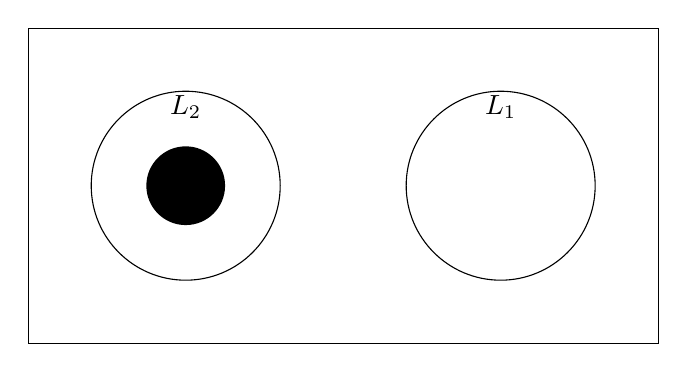
\begin{tikzpicture}
    % Outer rectangle
    \draw (0,0) rectangle (8,4);
    
    % Left egg shape with filled circle
    \draw (2,2) circle [x radius=1.2cm, y radius=1.2cm];
    \fill (2,2) circle [radius=0.5cm];
    
    % Right egg shape
    \draw (6,2) circle [x radius=1.2cm, y radius=1.2cm];   
    
    % Labels
    \node at (2,3) {$L_2$};
    \node at (6,3) {$L_1$};

\end{tikzpicture}

Consider the above image, the loop \( L_1 \) encloses a region outside the loop \(L_2 \) and the black part inside the loop \( L_2 \) denotes a region that has been cut off from the rectangle. Clearly the \(L_1\) loop can be shrunk to a point but the other one can't be shrunk to a point. Also these two loops cannot cross each other. 

The above is the study of Homotopy in Topology. Homotopy allows us to understand when two shapes or spaces can be continuously deformed into each other without tearing or gluing. It is a way of transforming one continuous function into another in a continuous manner. 

\begin{theorem}
    Two continuous functions \( f, g: X \rightarrow Y \) between topological spaces \( X \) and \( Y \) are said to be homotopic if there exists a continuous map \( H: X \times [0,1] \rightarrow Y \) such that:
\[ H(x, 0) = f(x) \]
\[ H(x, 1) = g(x) \]
for all \( x \in X \). The map \( H \) is called a homotopy between \( f \) and \( g \).
\end{theorem}

\subsection{Paths in Topology}

Let's move away from this for a moment and rethink our definition of path. 
\begin{theorem}
    A path from \( x_0 \in S \) to \( x_1 \in S \) in a topological space (S,U) is a continuous map \( \alpha(t): [0,1] \to S \) where \([0, 1]\) is the closed unit interval in the real numbers \(\mathbb{R}\). Such that 
    \[ \alpha(0) = x_0 \]
    \[ \alpha(1) = x_1\]
\end{theorem}

To be fair path is not an image but a function. We have the arbitrary freedom to chose our function but that has to map between topological space. 

\begin{theorem}
    A topological space \( S \) is said to be path-connected if for any two points \( x_0, x_1 \in S \), there exists a path \(\alpha\) such that \(\alpha(0) = x_0\) and \(\alpha(1) = x_1\). In other words, any two points in the space can be connected by a continuous path.
\end{theorem}

Now if a space is path connected then it is connected. Converse is not true. A space can be connected but not path connected. 

\subsection{Loops in Topology}
Now we move onto loops. Loops in topology is a closed path. Basically the starting and ending points/ sets are the same elements. 

\begin{theorem}
A \textit{closed path} or \textit{loop} in \(\mathcal{S}\) at \(x_0\) is a path \(\alpha(t)\) for which \(x_0 = x_1\), that is, \(\alpha(0) = \alpha(1) = x_0\). The loop is said to be \textit{based} at \(x_0\).
\end{theorem}

\begin{figure}
\centering
\begin{tikzpicture}

% Left circle
\draw (0,0) circle (1.5cm);
\node at (0,-1.7) {$t=0$};
\fill (0,-1.5) circle (0.05cm);
\node at (0,2) {$t=1/2$};
\node at (2.2,0) {$t=1/4$};
\node at (-2.2,0) {$t=3/4$};

% Arrow
\draw[->, thick] (2.3,0.2) to[out=30,in=150] node[above] {$\alpha(t)$} (4,0);

% Right shape
\begin{scope}[xshift=6cm]
\draw (0,0) to[out=90,in=180] (1,1) to[out=0,in=90] (2,0) to[out=270,in=0] (1,-1) to[out=180,in=270] cycle;
\fill (0,0) circle (0.05cm);
\node[anchor=north east] at (0,0) {$\alpha(0)=x_0$};
\draw (-2,-2) rectangle (2.5,1.5);
\end{scope}

\end{tikzpicture}
\caption{A based loop in a topological space $S$.}
\label{fig:based-loop}
\end{figure}

The idea of based at \( x_0 \) is very important. To multiply two loops we must have the condition that they are based at the same point. Otherwise they cannot be multiplied. We should also be careful in dealing the the \( \alpha(t) \). from the above definition. This is basically a space or collection of all possible functions or mappings. So we can have multiplie loops for the same based. 

\subsection{Loop Multiplication}
In topology, particularly in the study of the fundamental group, the multiplication of loops involves concatenating two loops to form a new loop, which in turn provides a group structure to the set of loops based at a given point. The formal definition is 

\begin{theorem}
Given a topological space \( X \) and a base point \( x_0 \in X \), let \(\alpha\) and \(\beta\) be two loops based at \( x_0 \). This means both \(\alpha\) and \(\beta\) are continuous maps \(\alpha, \beta: [0, 1] \to X\) such that \(\alpha(0) = \alpha(1) = x_0\) and \(\beta(0) = \beta(1) = x_0\).

The multiplication (or concatenation) of these loops, denoted \(\alpha * \beta\), is a new loop based at \( x_0 \) defined as follows:

\[
(\alpha * \beta)(t) = 
\begin{cases} 
\alpha(2t) & \text{for } 0 \leq t \leq \frac{1}{2}, \\
\beta(2t - 1) & \text{for } \frac{1}{2} < t \leq 1.
\end{cases}
\]
\end{theorem}

Why is it written like that. Its for abstraction and a more general handle on functions. 
For \( t \) in the first half of the interval \([0, 1]\), the loop \(\alpha * \beta\) follows the path of \(\alpha\) twice as fast (since \( \alpha(2t) \) covers the entire loop \(\alpha\) as \( t \) goes from \( 0 \) to \( \frac{1}{2} \)).
- For \( t \) in the second half of the interval \([0, 1]\), the loop \(\alpha * \beta\) follows the path of \(\beta\) twice as fast (since \( \beta(2t - 1) \) covers the entire loop \(\beta\) as \( t \) goes from \( \frac{1}{2} \) to \( 1 \)). So each of the \( \alpha, \beta \) individually obey the previous definitions. 

The inverse is also non-intuitive. Assuming the t value the \( \alpha(t) \) moves whatever it is in time t. Whereas, \( \alpha^{-1}(t) \) takes it back in time. So 

\[ \alpha^{-1}(t) = \alpha(1-t) \]

\subsection{Homotopy of Paths}

\begin{theorem}
    In topology, two paths \(\gamma_0\) and \(\gamma_1\) in a topological space \(X\), both starting at a point \(x_0\) and ending at a point \(x_1\), are said to be homotopic if one can be continuously deformed into the other. Formally, paths \(\gamma_0, \gamma_1: [0, 1] \to X\) are homotopic if there exists a continuous map \(H: [0, 1] \times [0, 1] \to X\) such that:

\[
H(t, 0) = \gamma_0(t), \quad H(t, 1) = \gamma_1(t) \quad \text{for all} \ t \in [0, 1],
\]

and

\[
H(0, s) = x_0, \quad H(1, s) = x_1 \quad \text{for all} \ s \in [0, 1].
\]

The map \(H\) is called a homotopy between \(\gamma_0\) and \(\gamma_1\).

\end{theorem}

Imagine stretching and bending a path \(\gamma_0\) to transform it into another path \(\gamma_1\), without breaking or lifting it from the space \(X\). This continuous deformation process is what a homotopy captures.

\begin{enumerate}
    \item \textbf{Reflexivity}: Every path is homotopic to itself.
    \item \textbf{Symmetry}: If \(\gamma_0\) is homotopic to \(\gamma_1\), then \(\gamma_1\) is homotopic to \(\gamma_0\).
    \item \textbf{Transitivity}: If \(\gamma_0\) is homotopic to \(\gamma_1\) and \(\gamma_1\) is homotopic to \(\gamma_2\), then \(\gamma_0\) is homotopic to \(\gamma_2\).
\end{enumerate}

\subsection{Homotopy of loops}

\begin{theorem}
A loop is a special kind of path that starts and ends at the same point, called the base point. Two loops \(\alpha_0\) and \(\alpha_1\) based at a point \(x_0\) in a topological space \(X\) are said to be homotopic if there exists a continuous map \(H: [0, 1] \times [0, 1] \to X\) such that:

\[
H(t, 0) = \alpha_0(t), \quad H(t, 1) = \alpha_1(t) \quad \text{for all} \ t \in [0, 1],
\]

and

\[
H(0, s) = H(1, s) = x_0 \quad \text{for all} \ s \in [0, 1].
\]

The map \(H\) is called a homotopy between \(\alpha_0\) and \(\alpha_1\).
\end{theorem}

For loops, the homotopy provides a way to continuously deform one loop into another while keeping the base point fixed. Imagine taking a rubber band looped around a fixed peg at \(x_0\) and transforming its shape continuously without lifting it off the peg.

Consider the unit circle \(S^1\). Any loop based at a point on the circle can be thought of as a map \(\alpha: [0, 1] \to S^1\) with \(\alpha(0) = \alpha(1)\). The loop that winds around the circle once counterclockwise is homotopic to the loop that winds around it once clockwise, but they belong to different homotopy classes if the winding numbers (how many times they wrap around the circle) are considered.

A clearer example would be two fixed points on a circle. We can pass a circle and if done properly we can fit a parabola or ellipse as well. All of these are then termed homotopic. 
They start and end at the same base point. 

Mathematically, if two loops \( \alpha \& \beta \) are homotopic to each other then, 

\[ \alpha \dot \sim \beta \]

homotopy is an equivalence relation. 

\begin{theorem}

\begin{enumerate}
    \item \textbf{Reflexivity}:
    \begin{itemize}
        \item Any loop is homotopic to itself. Mathematically, \(\alpha \dot \sim \alpha\).
    \end{itemize}

    \item \textbf{Symmetry}:
    \begin{itemize}
        \item If loop \(\alpha\) is homotopic to loop \(\beta\), then loop \(\beta\) is homotopic to loop \(\alpha\). Mathematically, if \(\alpha \dot \sim \beta\), then \(\beta \dot \sim \alpha\).
    \end{itemize}

    \item \textbf{Transitivity}:
    \begin{itemize}
        \item If loop \(\alpha\) is homotopic to loop \(\beta\) and loop \(\beta\) is homotopic to loop \(\gamma\), then loop \(\alpha\) is homotopic to loop \(\gamma\). Mathematically, if \(\alpha \dot \sim \beta\) and \(\beta \dot \sim \gamma\), then \(\alpha \sim \gamma\).
    \end{itemize}

    \item \textbf{Continuous Deformation}:
    \begin{itemize}
        \item Two loops \(\alpha\) and \(\beta\) are homotopic if there exists a continuous function \(H: S^1 \times [0, 1] \to X\) such that:
        \begin{itemize}
            \item \(H(s, 0) = \alpha(s)\) for all \(s \in S^1\),
            \item \(H(s, 1) = \beta(s)\) for all \(s \in S^1\),
            \item \(H(s, t)\) is continuous in both \(s\) and \(t\).
        \end{itemize}
    \end{itemize}

    \item \textbf{Base Point Preservation}:
    \begin{itemize}
        \item In the context of loops in a pointed space \((X, x_0)\), homotopy between loops must preserve the base point. This means that the base point \(x_0\) must remain fixed throughout the deformation:
        \begin{itemize}
            \item \(H(x_0, t) = x_0\) for all \(t \in [0, 1]\).
        \end{itemize}
    \end{itemize}

\end{enumerate}
    
\end{theorem}

To define a class of loops which are all homotopic to some loop \( \alpha \) is given by the notation \( [\alpha] \)


\subsection{Fundamental Group}

The \textbf{fundamental group} of a topological space \( S \) with a chosen base point \( x_0 \) is a mathematical structure that reflects the different ways in which one can traverse loops in the space starting and ending at \( x_0 \). It is denoted as \( \pi_1(S, x_0) \).


Formally, the fundamental group \( \pi_1(S, x_0) \) is the set of all equivalence classes of loops based at \( x_0 \), where two loops are considered equivalent if one can be continuously deformed into the other (i.e., they are homotopic):

\[
\pi_1(S, x_0) = \left\{ [\alpha] \mid \alpha(t) \text{ is a loop in } S \text{ based at } x_0 \right\}
\]

This is a group cause it has the following properties. 
\begin{enumerate}
    \item \textbf{Closure}: \[  [\alpha] \in \pi_1, \quad [\beta] \in \pi_1 \implies [\alpha] \star [\beta] = [\alpha \star \beta] \in \pi_1 \]

    \item \textbf{Identity}:  \([i]\) is the equivalence class of loops homotopic to the constant loop at \(x_0\). Clearly
        \[
        [\alpha] \star [i] = [i] \star [\alpha] = [\alpha \star i] = [\alpha]
        \]
        for all \([\alpha]\).

    \item \textbf{Inverse}:  \[
    [\alpha]^{-1} = [\alpha^{-1}], \text{ because }   \]
    \[  [\alpha]^{-1} \star [\alpha] = [\alpha^{-1} \star \alpha] = [i] \]

    \item \textbf{Associativity}: \[ ([\alpha] \star [\beta]) \star [\gamma] = [\alpha] \star ([\beta] \star [\gamma]) \]
\end{enumerate}

Also \(  [\alpha] \star [\beta] \neq [\beta] \star [\alpha] \) meaning this is not an Abelian Group. 

\subsubsection*{Examples}

\begin{itemize}
    \item \textbf{Simply Connected Spaces}: A space is simply connected if every loop can be contracted to a point. For such spaces, the fundamental group is trivial, consisting only of the identity element. An example is \(\mathbb{R}^n\) for \(n \geq 1\).

    \item \textbf{Circle \(S^1\)}: The fundamental group of the circle \(S^1\) is isomorphic to the integers \(\mathbb{Z}\). Each integer \(n\) corresponds to the loop that winds around the circle \(n\) times.
\end{itemize}

To proceed further, we will find it useful to define the product operation even on paths which are \textit{not} closed, namely, paths \(\alpha(t)\) such that \(\alpha(0)\) and \(\alpha(1)\) are distinct. 

\begin{theorem}
The \textit{product} of two open paths \(\alpha(t)\) and \(\beta(t)\) is defined only if \(\alpha(1) = \beta(0)\), in other words, if the final point of \(\alpha\) is the same as the initial point of \(\beta\), and is given by \(\gamma = \alpha \star \beta\) where:
\[
\gamma(t) = 
\begin{cases} 
\alpha(2t), & 0 \leq t \leq \frac{1}{2} \\
\beta(2t - 1), & \frac{1}{2} \leq t \leq 1
\end{cases} \quad 
\]

\end{theorem}

Here, the initial point of the product path \(\alpha \star \beta\) is the initial point of \(\alpha\), and the final point of \(\alpha \star \beta\) is the final point of \(\beta\).

Now we look to the fundamental groups once again. In principle this group depends on the base point with respect to which it is defined. Thus, \(\pi_1(S, x_0)\) is a different group from \(\pi_1(S, x_1)\) for \(x_0 \neq x_1\). But in fact under very general conditions the two are the same. 

To specify what we mean by two groups being the "same", let us first define the concept of "homomorphism" between groups (not to be confused with "homeomorphism" between topological spaces!). This is a mapping from one group to another which preserves the group operations. 

\begin{theorem}
    
If \(G\) and \(H\) are two groups, a \textit{homomorphism} \(\phi: G \to H\) is a map \(g \in G \rightarrow \phi(g) \in H\) such that:
\[
\begin{aligned}
&\phi: g^{-1} \in G \implies \phi(g^{-1}) = (\phi(g))^{-1} \in H \\
&\phi: g_1 \cdot g_2 \in G \implies \phi(g_1 \cdot g_2) = \phi(g_1) \cdot \phi(g_2) \in H \\
&\phi: i \in G \implies \phi(i) = i' \in H
\end{aligned}
\]
    
\end{theorem}

Homomorphism preserves group multiplication. We cannot say from homomorphism that G and H are the same group. They can or cannot be the same group. But there is a stronger condition called Isomorphism. 

\begin{theorem}
    A homomorphism \(\phi\) is an \textit{isomorphism} if it is also bijective (one-to-one and onto). If an isomorphism exists between two groups, the groups are said to be \textit{isomorphic}, and can be thought of as completely equivalent to each other.    
\end{theorem}

If there exists an isomorphism between G \& H, then effectively G \& H are the same group. So in other words they can be transformed onto one other. 

Now we can show the following 

\begin{theorem}
    If a topological space \( S \) is \textit{path-connected} then \(\pi_1(S, x_0)\) and \(\pi_1(S, x_1)\) are isomorphic as groups.

\textbf{Proof:} 
Consider \(\alpha(t)\) based at \(x_0\) along with its equivalence class \([\alpha] \in \pi_1(S, x_0)\). Let \(\gamma(t)\) be an open path from \(x_0\) to \(x_1\). Now define a map
\[
\phi : \pi_1(S, x_0) \to \pi_1(S, x_1) \quad \]
by
\[
\phi([\alpha]) = [\gamma^{-1} \star \alpha \star \gamma] \quad \]
Clearly \([\alpha] \in \pi_1(S, x_0) \implies \phi([\alpha]) \in \pi_1(S, x_1)\). And moreover this is an isomorphism. For example, the product law holds:
\[
\begin{aligned}
\phi([\alpha] \star [\beta]) &= \phi([\alpha \star \beta]) \\
&= [\gamma^{-1} \star \alpha \star \beta \star \gamma] \\
&= [\gamma^{-1} \star \alpha \star \gamma \star \gamma^{-1} \star \beta \star \gamma] \\
&= \phi([\alpha]) \star \phi([\beta]) \quad 
\end{aligned}
\]
with \([\alpha], [\beta] \in \pi_1(S, x_0)\). 

\end{theorem}

Similarly one can check the other properties of a homomorphism, as well as the fact that this map is bijective which finally makes it an isomorphism.

Because of the above theorem, for path-connected spaces we denote the fundamental group as \(\pi_1(S)\) instead of \(\pi_1(S, x_0)\). It must be kept in mind, however, that in the process of finding \(\pi_1\) we must always work with loops based at some (arbitrary) point \(x_0\). The final result for \(\pi_1\) will then be independent of \(x_0\).

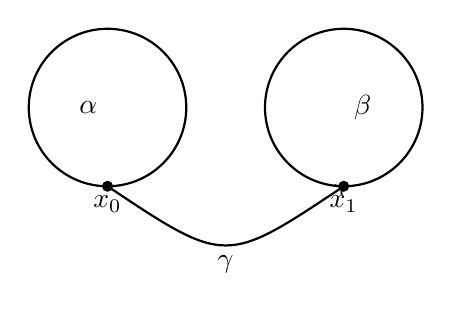
\begin{tikzpicture}
    % Draw the loops
    \draw[thick] (0,0) circle(1) node[left] {$\alpha$};
    \draw[thick] (3,0) circle(1) node[right] {$\beta$};
    
    % Draw the points
    \fill (0,-1) circle(2pt) node[below] {$x_0$};
    \fill (3,-1) circle(2pt) node[below] {$x_1$};
    
    % Draw the path gamma
    \draw[thick,->] (0,-1) .. controls (1.5,-2) .. (3,-1) node[midway, below] {$\gamma$};
\end{tikzpicture}

To understand what just happened we consider the terminologies once more. A path-connected space is a type of space where any two points can be joined by a continuous path. Whereas fundamental group \(\pi_1\) represents different "shapes" of loops that can be drawn from a starting point (base point) in the space and then return to the starting point without crossing edges or boundaries. These loops are looked at up to deformation, meaning one loop can be "stretched" or "squeezed" but not broken, into another.

The above theorem states that if you have a path-connected space \(S\), the fundamental group at any two points \(x_0\) and \(x_1\) in \(S\) are essentially the same, or in mathematical terms, "isomorphic." This isomorphism means there's a way to convert loops based at \(x_0\) to loops based at \(x_1\) without losing any fundamental properties of those loops. The way loops are transformed between two points involves "dragging" them along a path \(\gamma\) from \(x_0\) to \(x_1\).

In the diagram two loops \(\alpha\) and \(\beta\) based at points \(x_0\) and \(x_1\) respectively are connected by a path \(\gamma\). The transformation (or map) \(\phi\) defined in the proof essentially takes a loop at \(x_0\), drags it to \(x_1\) using \(\gamma\), then drags it back to \(x_0\), ensuring that the loop's nature remains unchanged. This dragging involves tracing the path to \(x_1\) (using \(\gamma\)), following the loop, and then coming back via the reverse path (\(\gamma^{-1}\)).

\subsection{Homotopy Types} 
The homotopy concept extends naturally to pairs of maps between any two topological spaces.

\begin{theorem}

 Let \(S\) and \(T\) be two topological spaces. For two continuous functions
\[
f_0: S \rightarrow T \quad \text{and} \quad f_1: S \rightarrow T,
\]
we say \(f_0\) and \(f_1\) are \textit{homotopic} if there exists a continuous map
\[
F: S \times [0, 1] \rightarrow T,
\]
such that the following conditions hold:
\[
F(x, 0) = f_0(x) \quad \text{and} \quad F(x, 1) = f_1(x).
\]
\end{theorem}

In the particular case where \(S\) is the closed interval \([0, 1]\), homotopy of functions simplifies to homotopy of paths or loops, but it's important to note that these do not rely on a fixed base point. Hence, we use the symbol \(\sim\) to denote the homotopy of functions described here, which should not be confused with based homotopy of loops denoted by the same symbol in other contexts.

Exploring homotopy between maps in various topological spaces helps us uncover properties shared between those spaces, which may not be immediately apparent.

Now we can define the homotopy of two topological spaces 

\begin{theorem}
Two topological spaces \( S \) and \( T \) belong to the same \textit{homotopy type} if there are continuous functions 
\[
f: S \rightarrow T \quad \text{and} \quad g: T \rightarrow S
\]
such that the compositions \( f \circ g \) and \( g \circ f \) are homotopic to the identity maps on \( T \) and \( S \) respectively. We denote these conditions as:
\[
f \circ g: T \to T \sim \text{i}_T \quad \text{and} \quad g \circ f: S \to S \sim \text{i}_S,
\]
where \( \text{i}_T \) and \( \text{i}_S \) are the identity maps on \( T \) and \( S \).

\end{theorem}

This characteristic of having the same homotopy type ensures that the fundamental groups of \( S \) and \( T \), denoted \( \pi_1(S) \) and \( \pi_1(T) \), are isomorphic. 

\begin{theorem}
If \( S \) and \( T \) are path-connected spaces with the same homotopy type, then their fundamental groups are isomorphic:
\[
\pi_1(S) \cong \pi_1(T).
\]    
\end{theorem}

This isomorphism indicates a deep connection between the spaces in terms of their loop structures and overall topology, despite potential differences in their geometries.

\begin{theorem}
If \( S \) and \( T \) are homeomorphic as topological spaces, then they share the same homotopy type, and consequently, their fundamental groups \( \pi_1 \) are identical. This follows because homeomorphism involves a pair of continuous maps \( f: S \to T \) and \( g: T \to S \) such that \( g = f^{-1} \), satisfying:
\[
f \circ g = \text{i}_T, \quad g \circ f = \text{i}_S.
\]
This establishes that \( S \) and \( T \) are homotopy equivalent.    
\end{theorem}
Now why do we need topology. Answer becomes apparant from the above discussion. Homotopy is topological invariant. Two spaces which are topologically equivalent (homeomorphic) have the same homotopy properties. However, the converse is not necessarily true. Two topological spaces may have the same \( \pi_1 \), but this does not imply that they are homeomorphic. 

We will need a few more definitions. Those are given below. 

\begin{theorem}
\textbf{1. } A Topological space is \textit{contractible} if it is homotopy equivalent to a single point.  

\textbf{2. } A topological space \( S \) is called \textit{simply connected} if its fundamental group \( \pi_1(S) \) is trivial, i.e., \( \pi_1(S) = \{i\} \), where \( i \) is the identity element. If \( \pi_1(S) \) contains more than the identity element, the space is \textit{multiply connected}.

\end{theorem}

Simply connected spaces are characterized by the absence of nontrivial loops: all loops can be continuously deformed into a point within the space. For a contractible space \( S \), the fundamental group \( \pi_1(S) \) is trivial, i.e., \( \pi_1(S) = \{i\} \). Therefore, such a space is simply connected. However, the converse is not always true; a simply connected space need not be contractible. We will explore this through examples below.

some examples to check homotopy and contractible spaces. 

\textbf{Example 1:} $\mathbb{R}^n$ is a Contractible Space

To show that $\mathbb{R}^n$ is a contractible space, we need to demonstrate that there exists a homotopy between the identity map on $\mathbb{R}^n$ and a constant map. A topological space is defined as contractible if it is homotopy equivalent to a point.

Here's how we can construct such a homotopy for $\mathbb{R}^n$:

Let $f: \mathbb{R}^n \to \mathbb{R}^n$ be the identity map, $f(x) = x$, and let $g: \mathbb{R}^n \to \mathbb{R}^n$ be a constant map, $g(x) = x_0$ for some fixed $x_0 \in \mathbb{R}^n$.

We need to find a continuous function $H: \mathbb{R}^n \times [0, 1] \to \mathbb{R}^n$ such that:
\begin{enumerate}
    \item $H(x, 0) = f(x) = x$ for all $x \in \mathbb{R}^n$,
    \item $H(x, 1) = g(x) = x_0$ for all $x \in \mathbb{R}^n$.
\end{enumerate}


Define $H$ by:
\[ H(x, t) = (1 - t)x + tx_0 \]
where $x \in \mathbb{R}^n$ and $t \in [0, 1]$.

\begin{itemize}
    \item \textbf{Continuity}: The map $H$ is clearly continuous as it is a linear combination of continuous functions $x$ and $x_0$, and scalar multiplication and addition in $\mathbb{R}^n$ are continuous operations.
    \item \textbf{Boundary Conditions}:
    \begin{itemize}
        \item At $t = 0$, $H(x, 0) = (1 - 0)x + 0 \cdot x_0 = x$, which is the identity map.
        \item At $t = 1$, $H(x, 1) = (1 - 1)x + 1 \cdot x_0 = x_0$, which is the constant map.
\end{itemize}
\end{itemize}

Since such a homotopy $H$ exists, we can conclude that $\mathbb{R}^n$ is homotopy equivalent to a single point, which implies that $\mathbb{R}^n$ is a contractible space. This demonstrates that all loops in $\mathbb{R}^n$ can be continuously shrunk to a point, and thus $\mathbb{R}^n$ has trivial homotopy groups, confirming its contractibility.

\textbf{Example 2:} 2-Sphere $S^2$ is not contractible 

To discuss the contractibility of a topological space, one must demonstrate the possibility to continuously deform every point in the space into a single point, effectively reducing the entire space to a point.

\[
S^2 = \{(x,y,z) \in \mathbb{R}^3 \mid x^2 + y^2 + z^2 = 1\}.
\]

A potential strategy to contract $S^2$ could involve moving every point to the south pole along great circles. However, this approach encounters a critical issue at the north pole, which cannot be moved in any direction without disrupting the continuity of the map. This obstacle implies that $S^2$ cannot be contracted to a point.

Despite this, any loop on $S^2$, based at any point, can be continuously shrunk to a point. This property indicates that the fundamental group of $S^2$ is trivial:

\[
\pi_1(S^2) = \{i\}.
\]

Thus, while $S^2$ is simply connected, implying that there are no non-trivial loops, its inability to be contracted to a single point due to the obstruction at the poles demonstrates that $S^2$ is \textbf{not contractible}.

\textbf{Example 3:} Circle $S^1$ is not contractible 

Consider \( S^1 \) as the set of all points in \( \mathbb{R}^2 \) at a unit distance from the origin. \( S^1 \) is not contractible and possesses a non-trivial fundamental group.

Define a loop \( \alpha_n: [0,1] \rightarrow S^1 \) where \( \alpha_n \) wraps around the circle \( n \) times. For \( n > 0 \), the loop winds \( n \) times anticlockwise; for \( n < 0 \), it winds \( |n| \) times clockwise; and for \( n = 0 \), \( \alpha_0 \) is the constant loop at a point \( x_0 \in S^1 \).

The fundamental group \( \pi_1(S^1) \) can be visualized by considering the homotopy classes of these loops. Two loops \( \alpha_n \) and \( \alpha_m \) are distinct in homotopy if \( m \neq n \), reflecting different numbers of wrappings around the circle, which cannot be homotopically deformed into one another.

The group operation in \( \pi_1(S^1) \) corresponds to the concatenation of loops, leading to the relation:
\[
[\alpha_n] * [\alpha_m] = [\alpha_{n+m}],
\]
where the right-hand side represents a loop that winds \( n+m \) times around the circle. This operation exhibits the structure of the integers \( \mathbb{Z} \) under addition. Formally, we have an isomorphism:
\[
\pi_1(S^1) \cong \mathbb{Z}.
\]
This isomorphism maps the homotopy class \( [\alpha_n] \) to the integer \( n \), known as the winding number of the loop.

Since \( \pi_1(S^1) \) is isomorphic to \( \mathbb{Z} \) and not trivial, \( S^1 \) is not contractible. A contractible space would have a trivial fundamental group, which is clearly not the case here. The presence of multiple, non-homotopic loops arising from different numbers of wrappings around the circle illustrates the rich topological structure of \( S^1 \) and confirms its non-contractible nature.

The above basically states take a coin and try to wrap the circular side using a rubber band twice or thrice. Then the question is can the rubber band deform to a single point or to a single loop structure. Obviously no, It cannot be morphed into a single loop without cutting a part of the rubber band. That's the argument used to prove that the loops on $S^1$ are not homotopic thus not contractible. 

\section{Differentiable Manifolds-I}

\subsection{Idea of Manifolds}

A topological space is a set equipped with a structure that allows us to talk about continuity and connectedness. The simplest examples are lines (\(\mathbb{R}\)) and planes (\(\mathbb{R}^2\)). If two spaces are homeomorphic, they must share key topological properties, like dimension. Dimension is a topological property. Consider, \(\mathbb{R}\) and \(\mathbb{R}^2\). By deleting a point from both, \(\mathbb{R} \setminus \{0\}\) becomes two disjoint intervals (disconnected), while \(\mathbb{R}^2 \setminus \{0\}\) remains connected. This difference in behavior upon the removal of a point helps prove that they are not homeomorphic, meaning they do not have the same topological dimension. \(S^1\) and \(\mathbb{R}\) are not homeomorphic, nor are \(S^2\) and \(\mathbb{R}^2\), again through arguments involving connectivity after removing points. Though \(S^1\) and \(S^2\) are not globally homeomorphic to \(\mathbb{R}\) and \(\mathbb{R}^2\) respectively, they are locally homeomorphic. This means in small enough neighborhoods, these behave like Euclidean spaces of their respective dimensions. 

\begin{theorem}
Let \( M \) be a topological space. A \textit{chart} \( C \) on \( M \) is a collection \( (U, \phi, n) \) such that:
\begin{enumerate}
    \item[(i)] \( U \) is an open set of \( M \).
    \item[(ii)] \( \phi \) is a homeomorphism: \( U \subseteq M \rightarrow \phi(U) \subseteq \mathbb{R}^n \). (Thus, \( \phi(U) \) is open in \( \mathbb{R}^n \).)
    \item[(iii)] \( n \) is a positive integer, called the \textit{dimension} of the chart \( C \).
\end{enumerate} 

\end{theorem}
In plain language, a chart is a piece of the topological space, with a homeomorphism equating it to a piece of some Euclidean space. 

It is evident that \( \mathbb{R}^n \) comes with a preferred choice of coordinates, called \textit{Cartesian coordinates}, namely the \( n \) real numbers specifying each point. Now given a chart, each point on it can be labelled by considering the image of this point in \( \mathbb{R}^n \) and then using the Cartesian coordinates of that point.

\begin{theorem}
    
Given a chart \( C = (U, \phi, n) \), the \textit{coordinates} of a point \( p \in U \subseteq M \) are the Cartesian coordinates in \( \mathbb{R}^n \) of the point \( \phi(p) \) in \( \phi(U) \subseteq \mathbb{R}^n \). When we allow the points \( p \) to vary over \( U \), the Cartesian components of \( \phi(p) \) in \( \mathbb{R}^n \) define a set of \( n \) real-valued functions on \( U \subseteq M \) called \textit{coordinate functions}.
    
\end{theorem}

The concept of chart has enabled us to locally map a piece of a topological space to \( \mathbb{R}^n \). A function on this piece of the topological space can then be differentiated by simply differentiating, in the familiar sense, the components of the coordinate functions defined above.

In simpler terms, this definition is about how we can understand and analyze shapes that might be more complex than standard shapes like planes or spheres. The idea of a "chart" is a tool in mathematics that helps us map a piece of a complicated shape onto a simpler, flat space like \(\mathbb{R}^n\) (which could be a line, plane, or higher-dimensional space). 

Think of a chart as a way of flattening a small part of a curved surface so that it looks like a regular flat piece of paper. This allows us to use simple calculus, which we usually do on flat surfaces, even on curved surfaces. When we use a chart, each point on our original shape gets a set of coordinates, just like on a flat grid. These coordinates are what we call "coordinate functions." Since one chart can only cover a part of the whole shape, we use many such charts to cover the entire shape. This way, we can apply calculus everywhere on the shape, not just where one chart is. By using multiple charts to cover an entire shape, we ensure that we can perform calculus operations (like differentiation) across the whole surface, no matter how complex its geometry might be. 

\begin{theorem}
Let \( C_1 = (U_1, \phi_1, n) \) and \( C_2 = (U_2, \phi_2, n) \) be two charts on \( M \). Then \( C_1 \) and \( C_2 \) are ``\(C^\infty\)-compatible'' or simply ``compatible'' if:
\begin{enumerate}
    \item[(i)] \( U_1 \cap U_2 = \emptyset \), or
    \item[(ii)] the maps \( \phi_1 \circ \phi_2^{-1} : \phi_2(U_1 \cap U_2) \rightarrow \phi_1(U_1 \cap U_2) \) and \( \phi_2 \circ \phi_1^{-1} : \phi_1(U_1 \cap U_2) \rightarrow \phi_2(U_1 \cap U_2) \) are infinitely differentiable (\( C^\infty \)) functions.
\end{enumerate}    
\end{theorem}

\begin{figure}
    \begin{center}
        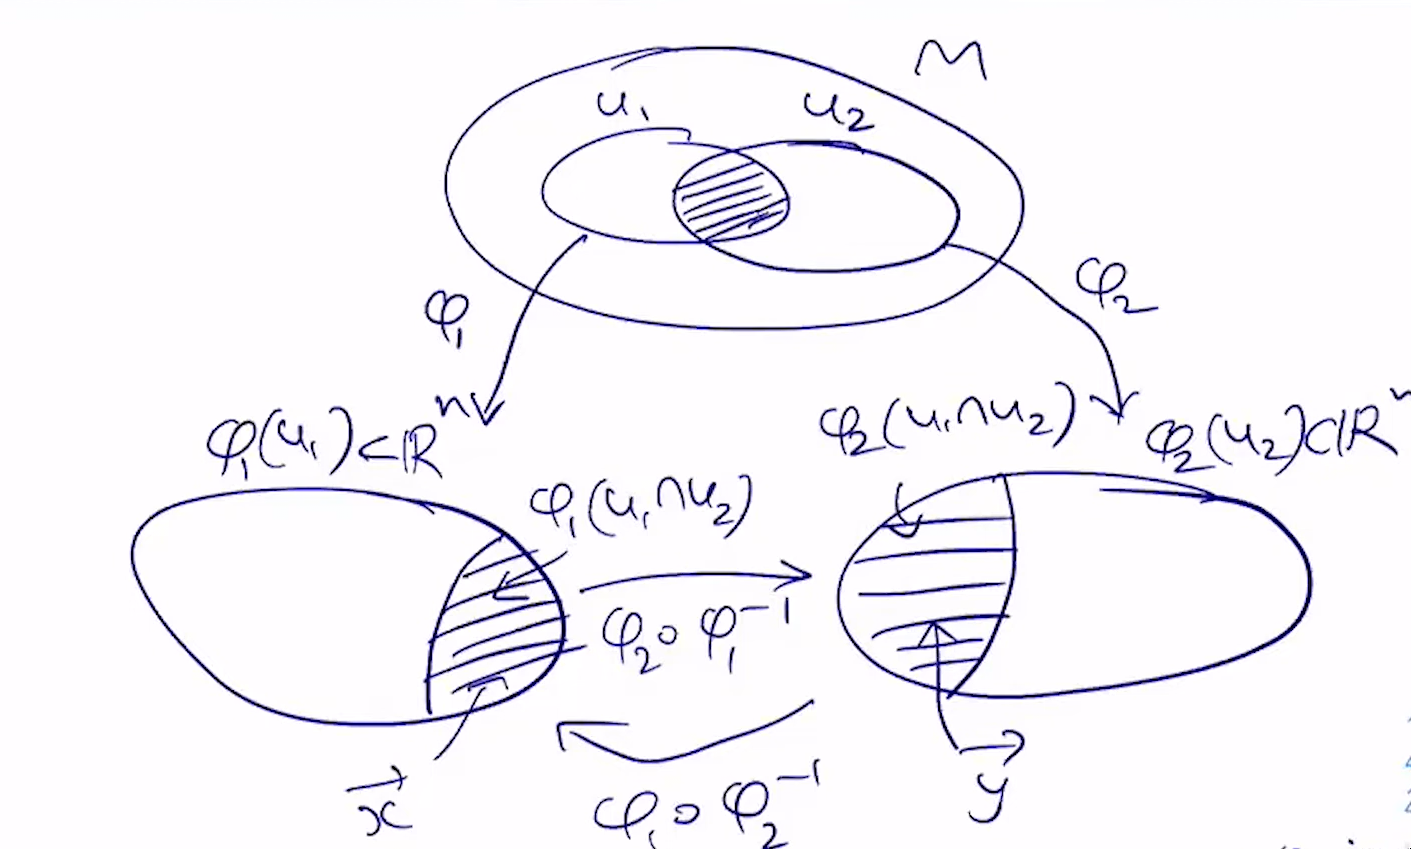
\includegraphics[width=0.95\textwidth]{figures/def_manifold.png}
    \end{center}
    \caption{Definition of a Manifold}\label{fig:definition_manifold}
\end{figure}

In the figure, consider that some person used the shaded region of the M space and converted/transformed or cut or whatever terminology is relevent, and gets the left part of the shaded region in $\phi_1(u_1)$ this is basically the same as saying that the person just wrote the physical law in terms of variable $\vec{x}$. Now another person can do the same thing maybe in a different coordinate system or different frame and will get the right portion $\vec{y}$. Since they are overlappong and are the same thing we now have a relation between two coordinates $\vec{x} \& \vec{y}$. They can now be transformed or differentiated. 

\begin{theorem}
    A \(C^\infty\)-atlas \( \mathcal{U} \) on a topological space \( M \) is a family of charts \( (U_\alpha, \phi_\alpha, n) \) which covers \( M \), so that \( \bigcup_\alpha U_\alpha = M \), such that all the charts in the family are mutually \(C^\infty\)-compatible.

    Two \(C^\infty\)-atlases are said to be \textit{compatible} (with each other) if every chart of one atlas is compatible with every chart of the other atlas.

\end{theorem}
A \(C^\infty\)-atlas on a topological space \(M\) is a collection of charts that together cover the entire space \(M\). Each chart in this collection maps a part of \(M\) into Euclidean space \(\mathbb{R}^n\). The superscript \(C^\infty\) indicates that the charts are smooth, meaning that the transition maps between any two overlapping charts are infinitely differentiable.

The map \(\phi_\alpha\) essentially provides a coordinate system for each part of the manifold. The union of all open sets \(U_\alpha\) in the atlas equals the entire manifold, ensuring no part of \(M\) is left out. The charts must smoothly align where they overlap. If you transition from one chart to another where they overlap, this transition must be smooth (infinitely differentiable).

Two \(C^\infty\)-atlases are considered compatible if every chart in one atlas is compatible with every chart in the other atlas. This means that for any pair of overlapping charts, one from each atlas, the transition map between them must be infinitely differentiable.

Compatibility is essential for defining a consistent structure on the manifold that doesn't depend on the choice of atlas. If two atlases are compatible, they essentially provide the same "smooth structure" to the manifold, allowing for a unified approach to calculus and analysis on \(M\).

An interesting property of atlases and charts are that for \(C^\infty\)-compatibility is an equivalence relation. It implies three key things:

1. \textbf{Reflexivity}: Every atlas is \(C^\infty\)-compatible with itself. The transition maps within a single atlas are, by definition of the atlas being a \(C^\infty\)-atlas, infinitely differentiable.

2. \textbf{Symmetry}: If atlas A is \(C^\infty\)-compatible with atlas B, then atlas B is \(C^\infty\)-compatible with atlas A. This means that if you can transition smoothly from charts in A to charts in B, the reverse transitions are also smooth.

3. \textbf{Transitivity}: If atlas A is \(C^\infty\)-compatible with atlas B, and atlas B with atlas C, then atlas A is \(C^\infty\)-compatible with atlas C. This ensures that smooth structures can be extended across multiple atlases, maintaining a consistent differentiable structure throughout.

But for charts, the key issue arises in the physical extent of the overlap and the specific transition functions used. Suppose \(A\) overlaps with \(B\) in one region and \(B\) overlaps with \(C\) in a different region. There may be no direct overlap between \(A\) and \(C\), or the overlap between \(A\) and \(C\) might involve different sections of these charts that were not "tested" via the transitions through \(B\). This can lead to situations where direct transitions between \(A\) and \(C\) are not smooth, even though transitions through \(B\) are smooth. 

\begin{theorem}
    A differentiable structure of class \(C^\infty\) on a topological space \(M\) is an equivalence class of \(C^\infty\)-compatible atlases on \(M\).     
\end{theorem}

It is always easier to study equivalence classes if we can find a unique representative of each class in some way, since this can then be used to label the class. We may pick a unique atlas out of each equivalence class of compatible atlases as follows: take the union of all atlases in a class and call it the \textit{maximal atlas}. Then a differentiable structure is just a choice of maximal atlas \(U\) on \(M\). This choice therefore labels the differentiable structure.

We are finally in a position to define a manifold.

\begin{theorem}
    A differentiable manifold is a Hausdorff topological space and an equivalence class of atlases.    
\end{theorem}

Now, what is going on? Lets start with the terminologies. 

A topological space is termed "Hausdorff" if any two distinct points in the space can be separated by disjoint open sets. This separation means that no two points can be arbitrarily close without being the same. A manifold is equipped with an atlas, which is a collection of charts that together cover the entire manifold. Each chart provides a way to coordinate or "chart" part of the manifold, typically mapping it to an open subset of Euclidean space (\(\mathbb{R}^n\)). An equivalence class of atlases refers to a group of atlases where any atlas in the group can be smoothly transformed into any other through their transition maps. This means all atlases in this class provide a consistent way to study the manifold’s structure, enabling calculus and other analyses.
It doesn't matter which atlas from the class you choose to use; they all describe the manifold in a way that is consistent with each other in terms of smoothness and differentiability.

Combining these two characteristics, the definition describes a space that not only has a straightforward and well-defined topological nature (Hausdorff) but also allows for smooth calculus operations anywhere on the manifold due to its differentiable structure (given by the equivalence class of \(C^\infty\) atlases).

\begin{theorem}
\textbf{Properties of Differential Manifolds}:
\begin{enumerate}
    \item It is locally Euclidean.
    \item It is locally compact (every point \( x \in M \) has a compact neighbourhood).
    \item An open subset \( U \subseteq M \) is itself a differentiable manifold, called an ``open submanifold''.
    \item The product of two manifolds is well-defined (using Cartesian products).
\end{enumerate}
\end{theorem}

\textbf{\(\mathbb{R}^n\) is a Differentiable Manifold}

1. \textbf{Locally Euclidean:} By definition, any point in \(\mathbb{R}^n\) has a neighborhood that looks exactly like \(\mathbb{R}^n\), fulfilling the locally Euclidean condition directly.

2. \textbf{Atlas and Charts:} For \(\mathbb{R}^n\), we can use a single chart covering the entire space where the chart map \(\phi\) is the identity map \(\phi: \mathbb{R}^n \rightarrow \mathbb{R}^n\)

3. \textbf{Smooth Compatibility:} Since we only have one chart, and it maps to itself by the identity function, the compatibility condition (smooth transitions between charts) is automatically satisfied.

4. \textbf{Hausdorff and Second-countable:} The space \(\mathbb{R}^n\) is Hausdorff as any two distinct points can be separated by disjoint open sets. It is second-countable as it has a countable basis (e.g., open balls with rational radii centered at points with rational coordinates).

Hence, \(\mathbb{R}^n\) is a differentiable manifold.

\textbf{Proving \(S^1\) is a Differentiable Manifold}

1.\textbf{Locally Euclidean:}  Each point on \(S^1\) (defined as \(S^1 = \{(x, y) \in \mathbb{R}^2 : x^2 + y^2 = 1\}\)) has a neighborhood that resembles an open interval in \(\mathbb{R}\), satisfying the locally Euclidean condition.

2. \textbf{Atlas and Charts:} We can cover \(S^1\) with two charts to avoid the coordinate singularity at one point (commonly taken at \( (1,0) \) and \((-1,0)\)):
   - Chart \(U_1 = S^1 \setminus \{(1,0)\}\) with coordinates given by the projection onto the y-axis, or an angular coordinate excluding the angle corresponding to \((1,0)\).
   - Chart \(U_2 = S^1 \setminus \{(-1,0)\}\) similarly defined.

3. \textbf{Smooth Compatibility:} The transition maps between these two charts (moving from one angular coordinate to another excluding different points) are smooth, involving simple arithmetic operations on the angles.

4.\textbf{Hausdorff and Second-countable:}  \(S^1\), as a subspace of \(\mathbb{R}^2\), inherits the Hausdorff property. It is also second-countable as it can be covered by a countable union of open arcs.

Thus, \(S^1\) is a differentiable manifold.

\subsection{Differentiation of functions} 

\begin{figure}
    \begin{center}
        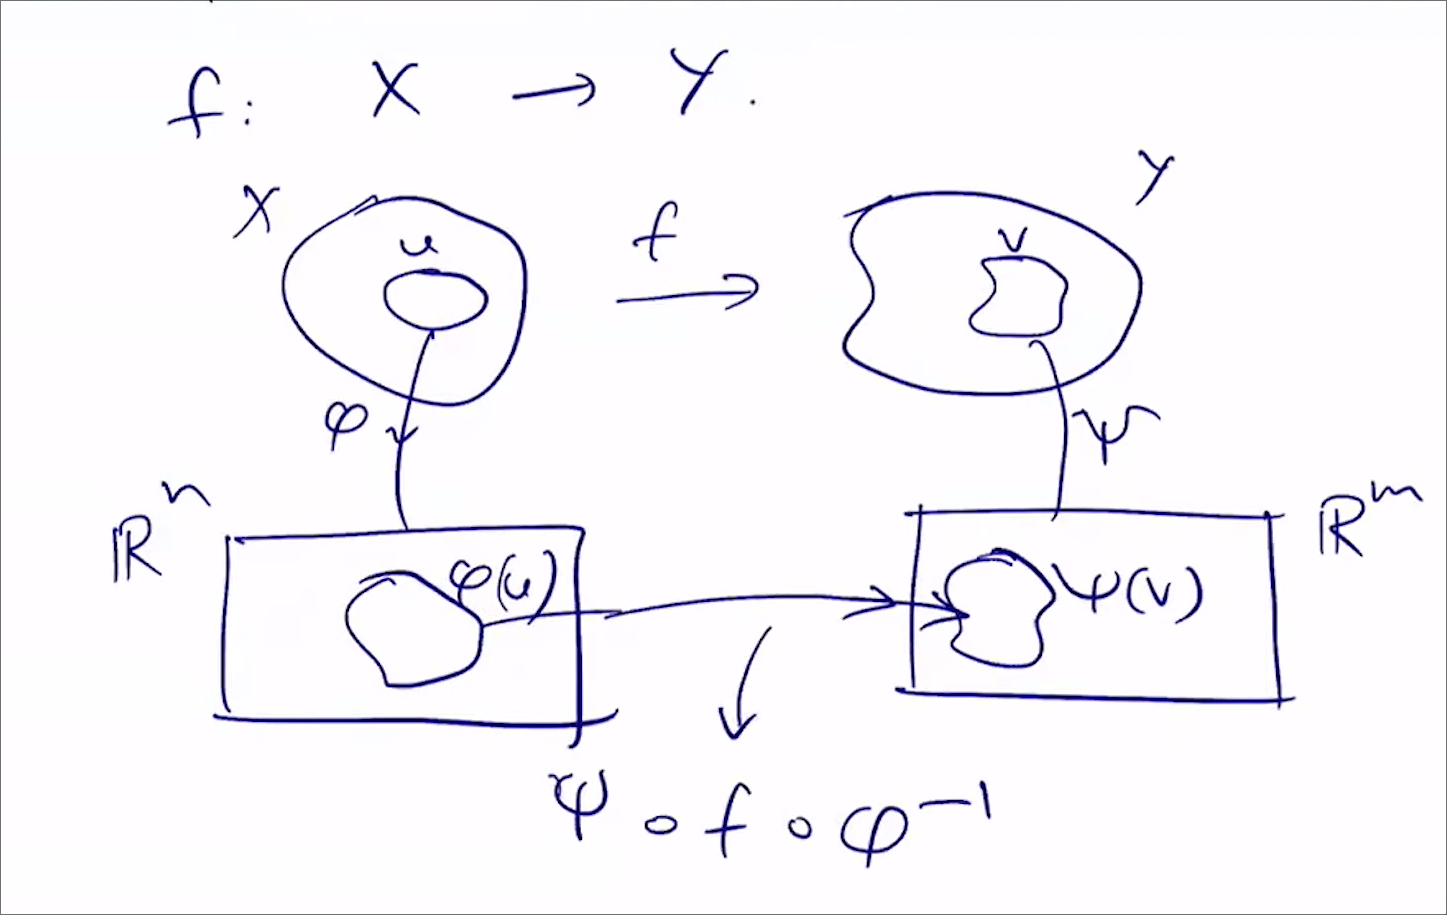
\includegraphics[width=0.95\textwidth]{figures/eq_manifolds.png}
    \end{center}
    \caption{}\label{fig:}
\end{figure}

In the context of manifolds, we define a function to be differentiable in a manner analogous to functions in Euclidean space. However, since manifolds may not have global coordinate systems, we rely on local coordinates provided by charts.

\begin{theorem}
A function \( f: X \to Y \) between manifolds is said to be differentiable if the function \(\psi \circ f \circ \phi^{-1} : \mathbb{R}^n \to \mathbb{R}^m\) is differentiable in the usual sense. Here, \(\phi\) and \(\psi\) are chart maps for manifolds \(X\) and \(Y\), respectively, translating manifold coordinates into Euclidean coordinates where standard calculus applies.
\end{theorem}

Diffeomorphisms are a special type of mapping between manifolds that not only preserve the structure of the manifolds but also allow for the smooth translation of geometric and analytic properties between them.

\begin{theorem}
    Two manifolds \(X\) and \(Y\) are said to be diffeomorphic if there exists a function \(f: X \to Y\) such that:
    \begin{enumerate}
        \item[(i)] \(f\) is a homeomorphism, ensuring a one-to-one, onto, and continuous mapping with a continuous inverse.
        \item[(ii)] Both \(f\) and \(f^{-1}\) are \(C^\infty\), meaning they are smooth; this includes having all derivatives exist and be continuous.
    \end{enumerate}
\end{theorem}

\subsection{Orientability}
Orientability of a manifold refers to the possibility of consistently defining what it means to be clockwise or counterclockwise across the entire manifold.

\begin{figure}
    \begin{center}
        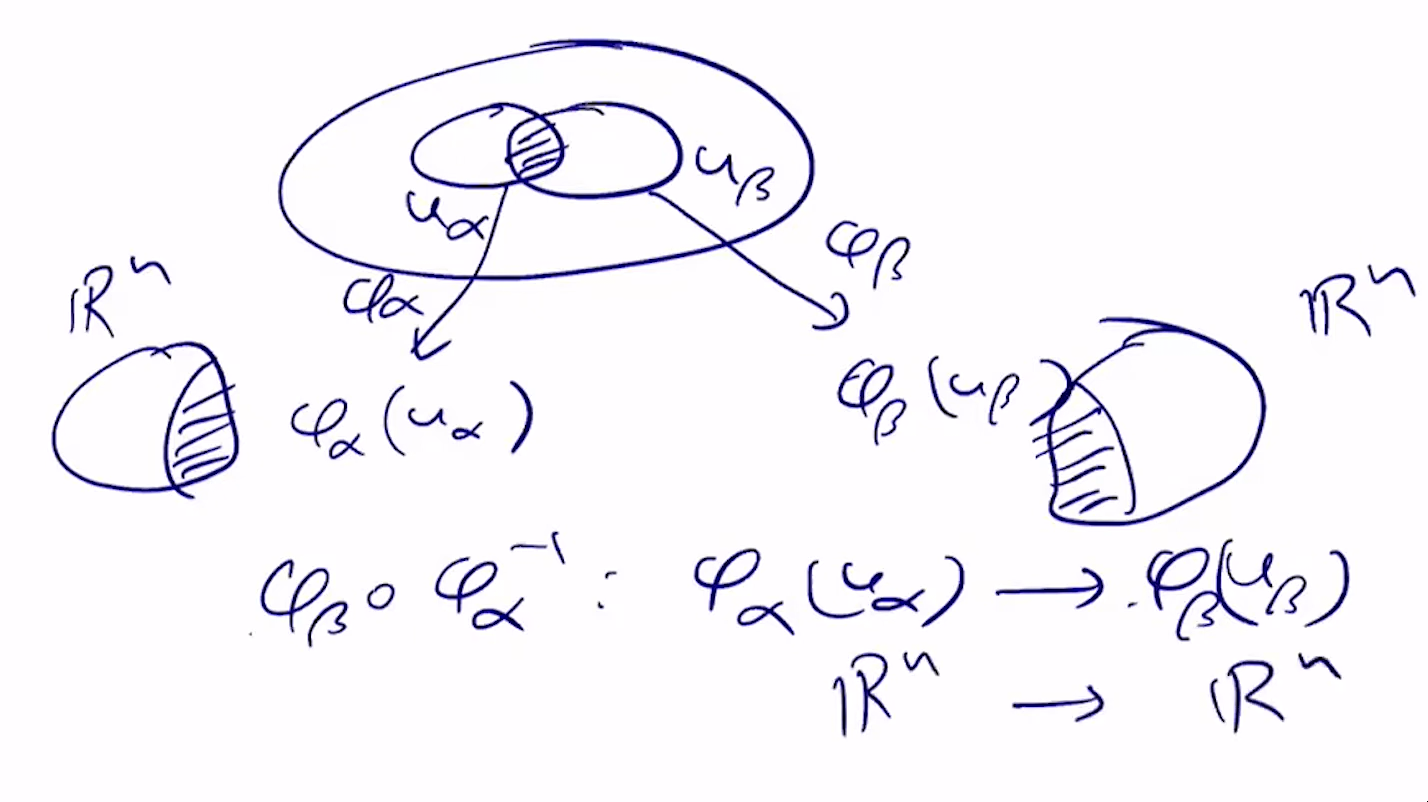
\includegraphics[width=0.95\textwidth]{figures/orientation.png}
    \end{center}
    \caption{}
\end{figure}

\begin{theorem}
    A manifold is \textit{orientable} if an atlas can be chosen such that for every overlap of charts, the transition map \(\phi_{\beta} \circ \phi_{\alpha}^{-1} : \mathbb{R}^n \rightarrow \mathbb{R}^n\) has a positive Jacobian determinant. This positive determinant indicates that orientation is preserved between overlapping charts.
\end{theorem}

\section{Calculus on manifolds}

While local regions of manifolds look like Euclidean space, the global topology can significantly differ. Ordinary calculus doesn't directly address how to define derivatives when the underlying space (manifold) can curve or loop back on itself.
How to handle calculations across manifold charts, where local Euclidean views must seamlessly connect through transition maps. Nor does it help in computing derivatives that respect the manifold's intrinsic geometry, which can be critical in physics for understanding phenomena like gravity or electromagnetism in curved spacetime. To address these issues, calculus on manifolds formalizes and extends the concepts of differentiation and integration to work in curved spaces. 

\subsection{Tangent Vectors and Tangent Space} 

The concept of a differentiable manifold is crucial because it allows us to apply calculus as we do in $\mathbb{R}^n$, thanks to local equivalence. To manage this, we employ coordinate charts to transition from manifold calculus to $\mathbb{R}^n$. The main complexity arises in transferring calculations between multiple charts that cover the manifold.

Consider a real-valued function $f : M \rightarrow \mathbb{R}$ on a manifold $M$. Within a coordinate patch, this function corresponds to a map $\mathbb{R}^n \rightarrow \mathbb{R}$. Changing the coordinate system alters the function representation:
\[
f' : y^i \in \mathbb{R}^n \rightarrow f'(y^i) \in \mathbb{R},
\]
where the transformation on overlapping charts for a different coordinate is defined by:
\[
f'(y^i) = f(x^i).
\]
Differentiating $f$ in a coordinate patch $\varphi_\alpha(U_\alpha)$ gives:
\[
\frac{\partial f}{\partial x^i} : \varphi_\alpha(U_\alpha) \rightarrow \mathbb{R}.
\]
Though $f$ is coordinate invariant, its derivatives transform differently:
\[
f'(y) = f(x) \Rightarrow \frac{\partial f'}{\partial y^i} = \frac{\partial f}{\partial x^i} \frac{\partial x^i}{\partial y^i} \neq \frac{\partial f}{\partial x^i}.
\]

To better grasp this, consider a parametrized curve $p(t) \subseteq M$, which in a coordinate patch maps to $x^i(t) \subseteq \mathbb{R}^n$. The tangent vector at $t_0$ is defined as $dx^i/dt |_{t=t_0}$, encapsulating the rate and direction of motion at that point. 

\begin{theorem}
In a coordinate patch, the tangent vector to a curve $p(t) \subseteq M$ is $dx^i/dt$, derived from the coordinates $x^i(t)$ of the curve's image $\varphi_\alpha(p(t))$.
\end{theorem}

Tangent vectors transform between overlapping patches as follows:
\[
\frac{dx^i}{dt} \rightarrow \frac{dy^i}{dt} = \frac{\partial y^i}{\partial x^j} \frac{dx^j}{dt},
\]
making the tangent vector's meaning invariant across different coordinates, a property known as "covariance". We simply mean the tangent is now in a coordinate-less representation. 

\textbf{Vector Space of Tangent Vectors:} Tangent vectors at a single point form a vector space. We can have a \( n>=1 \) number of tangents drawn in any direction. Combining tangent vectors from two intersecting curves $p(t)$ and $q(t)$ at $t_0$ generates a new vector:
\[
a^i(x_0) = \left[ \frac{dx^i}{dt} (p(t)) + \frac{dx^i}{dt} (q(t)) \right]_{t=t_0},
\]
This describes a straight line in $\mathbb{R}^n$:
\[
x^i(t) = x_0^i + a^i(x_0)t.
\]
Here \( x_0 \) is the image of the point \( p(0) \) on the manifold. This line can be mapped back to $M$, forming a new curve around the intersection point of $p(t)$ and $q(t)$, using $\varphi_\alpha^{-1}$.

\begin{theorem}
The set of all tangent vectors at a point $p \in M$ constitutes the tangent space $T_p(M)$.

Tangent vectors are constructed by:
\begin{enumerate}
    \item Choosing a point $x_0^i \in \mathbb{R}^n$ and defining a curve such that $\left. \frac{dx^i}{dt} \right|_{t=t_0} = a^i$.
    \item Lifting this curve to $M$ using $\varphi_\alpha^{-1}$.
    \item In another coordinate system, redefining the vector components to maintain consistency across transformations.
\end{enumerate}    
\end{theorem}

Combining the differentiation of functions with tangent vector analysis on $M$ provides a coordinate invariant definition of a tangent vector. The derivative of a function $f$ along a curve is a coordinate-independent differential:
\[
\frac{df}{dt} = \frac{df}{dx^i} \frac{dx^i}{dt} (p(t)),
\]

Thus, the derivative of $f$ along a curve, at some point, is expressed in terms of its gradient $\frac{\partial f}{\partial x^i}$ in the chosen coordinate system, contracted with the tangent vector at that point. But while both $\frac{\partial f}{\partial x^i}$ and $\frac{dx^i}{dt}$ are coordinate-dependent objects, when contracted together they give $\frac{df}{dt}$ which is manifestly coordinate independent. 

Now, 
\[
\frac{df}{dt} = \left[ \frac{dx^i}{dt} (p(t)) \right] \left[ \frac{\partial}{\partial x^i} \right] f.
\]
This operator, $\frac{dx^i}{dt} (p(t)) \frac{\partial}{\partial x^i}$, maps any $C^\infty$ functions on a manifold to a new functions on the curve and is termed a vector field when generalized over the manifold. The linearity and distribution over function multiplication define and characterize vector fields:
\[
X(fg) = (Xf)g + f(Xg).
\]

\subsection{Tensor Fields and differential forms} 

Let's start from the previous part. Vector at a point takes a function to a another function in the below manner. 

\[ X : f \to X f \]

Where we define the X in two ways. In the abstract way we mean the following 

\[ X(fg) = (Xf)g + f(Xg) \]

this is the product form. But in coordinates we say that $ X = a^i \frac{\partial}{\partial x^i}$. So its the gradient operator along some curve based on what we choose on the manifold. This is called vector at a point. But a vector field extends the idea in a differentiable way over the whole manifold. For example 

\[ X:f \to Xf \]
if X were to be a vector field that would mean X now sends to all over the manifold. Also all of these are now \( C^{\infty}\)

Now to define a tensor field. We first start the abstract manner. Let's take a collection of functions \( f_1 \cdot \cdot f_n\) and treat them as a n component vector. 
Now a tensor field of rank n which satisfies the product rule 

\begin{theorem}
    
 A tensor field of rank $n$ is a multilinear map
\begin{equation}
X : (f_1, \ldots, f_n) \to X(f_1, \ldots, f_n)
\end{equation}
satisfying
\begin{equation}
X((f_1, \ldots, f_n) \ast (g_1, \ldots, g_n)) = (X(f_1, \ldots, f_n)) \ast (g_1, \ldots, g_n) + (f_1, \ldots, f_n) \ast (X(g_1, \ldots, g_n))
\end{equation}

\end{theorem}
In coordinate system, we get 
\begin{equation}
a = a^{i_1 i_2 \ldots i_n}(x) \frac{\partial}{\partial x^{i_1}} \otimes \frac{\partial}{\partial x^{i_2}} \otimes \ldots \otimes \frac{\partial}{\partial x^{i_n}}
\end{equation}

The transformation law for the gradient can be found by chain rule. So requiring X to be coordinate independent givees us the law for $ a = a^{i_1 i_2 \ldots i_n}(x) $

So if i change the coordinate system \( x^i \to x^{i'} \) then  $ a^{i_1 i_2 \ldots i_n}(x) \to a^{i^{'}_1 i^{'}_2 \ldots i^{'}_n}(x) $ 
can be defined as 

\[ 
a'^{i_1 \ldots i_n}(x') = \frac{\partial x^{i_1}}{\partial x^{j_1}} \ldots \frac{\partial x^{i_n}}{\partial x^{j_n}} a^{j_1 \ldots j_n}(x)
\] 

these can be called the components of the tensor and X is the tensor. The above is called in contravariant tensor in physics term which is derived from old mathematical textbooks a modern way to represent it would be to call it components of a tensor field. 

Now suppose we have two \( C^\infty \) manifolds with a map 
\[ \phi:M \to N \] 
such that there is another function for which 
\[ f:N \to \mathbb{R} \]
So basically we now have a functional mapping of the form 
\[ f \circ \varphi :M \to \mathbb{R} \]
the above is a point wise map from M to N. We can define a general mapping of the form 
\[ \varphi_{*} : T_{p} (M) \to T_{\varphi(p)} (N) \]
Here \(T_{p}(M) \) denotes the tangest vector space at point p over the manifold M. So \( \varphi_{*}  \) is a map from tangent space on M at point p to the tangent space at the image point \( \varphi(p) \) over the manifold N. The map has the following property. 

\[ \varphi_{*} : X \in T_{p}(M) \to \varphi_{*}X \in T_{\varphi(p)}(N) \] 
Which by definition means that \( \varphi_{*}X \) is vector field on N which acts on functions f by the following process. 

\[ (\varphi_{*}X)f = X(f\circ \varphi) \]

\begin{theorem}
    If X,Y two vector fields on M and \( f : M \to \mathbb{R} \) then 
    \[ XYf = X(Yf) \]
    \[ YXf = Y(Xf) \] 

    Since they dont have to be the same we define \( [X,Y] \) is the vecor field whose action on a function \( f:M \to \mathbb{R} \) is 

    \[ [X,Y]f  = XYf - YXf \]
    this is also called the lie bracket or simply the commutator. 
\end{theorem}

In coordinates:
\begin{align*}
X &= a^i(x) \frac{\partial}{\partial x^i}, & Y &= b^i(x) \frac{\partial}{\partial x^i} \\
X(Yf) &= a^i \frac{\partial}{\partial x^i} \left( b^j \frac{\partial f}{\partial x^j} \right) \\
      &= a^i b^j \frac{\partial^2 f}{\partial x^i \partial x^j} + a^i \frac{\partial b^j}{\partial x^i} \frac{\partial f}{\partial x^j} \\
Y(Xf) &= b^j \frac{\partial a^i}{\partial x^j} \frac{\partial f}{\partial x^i} + b^j a^i \frac{\partial^2 f}{\partial x^j \partial x^i} \\
(XY - YX)f &= \left( a^i \frac{\partial b^j}{\partial x^i} - b^i \frac{\partial a^j}{\partial x^i} \right) \frac{\partial f}{\partial x^j} \\
[X,Y] &=c^{j}\frac{\partial f}{\partial x^j} 
\end{align*}

where \[ c^j (x) = a^i \frac{\partial b^j}{\partial x^i} - b^i \frac{\partial a^j}{\partial x^i} \]

This is how the lie bracket work. The components of the lie bracket are these combination of components of the original vector fields. This also has a geometric meaning. The vector fields mentioned above are supposed to generate a motion on those differentiable manifold along some curve. They can come from a particular curve or can be used to construct a particular curve. Either way they generate some sort of motion. So if i have X,Y two different vector fields. One will generate a motion along one curve and the other will generate a motion along some other curve. 

So a commutator is basically saying let me travel along a bit on one curve and then travel along the other curve for a bit. After that let's compare the results. So i move in two independent directions and the difference of those two will give me the lie bracket. 

Now let's talk about differential forms. 

\section{Differential forms}
We first start off with dual vectors. 

Given a vector space \( V \) with a basis \( \{e_i\} \) where \( i = 1, \ldots, n \), the dual vector space \( V^* \) is defined as the vector space generated by the dual basis \( \{e^i\} \), such that:
\[
\langle e^i, e_j \rangle = \delta^i_j
\]

For finite-dimensional vector spaces, \( V^* \) is isomorphic to \( V \). The pairing between elements of \( V \) and \( V^* \) leads to different properties for these spaces, which are influenced by their transformation properties under coordinate changes. The inner product remains invariant under certain transformations.

In this context, we want to focus on the dual of the tangent space, deriving the transformation laws for elements of this space to ensure coordinate invariance. This involves expressing elements of \( V \) and \( V^* \) in terms of their respective bases, and studying the behavior under coordinate transformations.

In general, elements of \( V \) and \( V^* \) can be expressed in terms of their respective bases:
\[
a = \sum_{i} a^i e_i \quad \text{in} \, V, \quad a' = \sum_{i} a'_i e^{i} \quad \text{in} \, V^*
\]

Then, the pairing between \( a' \) and \( a \) is given by:
\[
\langle a', a \rangle = a'_i a^j \langle e^i, e_j \rangle = a'_i a^i \quad (\text{summation implied})
\]
Thus, the pair \( a' \in V^*, a \in V \) gets mapped onto a real number, or in other words, \( \langle \cdot, \cdot \rangle \) is a bilinear map:
\[
V^* \otimes V \to \mathbb{R}
\]

There is an alternative way to look at this. For a given \( a' \in V^* \), we have a linear map
\[
\langle a', \cdot \rangle : V \to \mathbb{R}
\]
defined by
\[
\langle a', a \rangle : a \in V \mapsto \langle a', a \rangle \in \mathbb{R}
\]

Thus the dual vector space to \( V \) is the space of linear functionals on \( V \).


An important property of dual spaces is that if we have a map of vector spaces \( V, W \):
\[
f : V \to W
\]

then this induces a dual map in the opposite direction:
\[
f^* : W^* \to V^*
\]

If \( b' \in W^* \), then \( f^*b' \) acts on vector \( a \in V \) by:
\[
\langle f^*(b'), a \rangle: \to \langle f^*(b'), a \rangle = \langle b', f(a) \rangle
\]
In summary 

  \[
  \langle f^*(b'), a \rangle = \langle b', f(a) \rangle
  \]

Here the Left Side (\(\langle f^*(b'), a \rangle\)) is the evaluation of the functional \( f^*(b') \) at the vector \( a \) in \( V \). It produces a real number since \( f^*(b') \) is a functional in \( V^* \).
The right side (\(\langle b', f(a) \rangle\)) \( f(a) \) maps the vector \( a \) from \( V \) to \( W \), and then \( b' \) is evaluated at this new vector \( f(a) \) in \( W \). The equality shows that \( f^*(b') \) acting on \( a \) in \( V \) is equivalent to \( b' \) acting on the image of \( a \) under \( f \) in \( W \). This is fundamental in the definition of the dual map, where \( f^* \) effectively "pulls back" the functional \( b' \) along the map \( f \), allowing it to act directly on vectors in \( V \) as though they were in \( W \).

In the study of differentiable manifolds, we defined the tangent space \(T_p(M)\) at a point \(p\), with basis \(\frac{\partial}{\partial x^i}\). Now we will define its dual.

\begin{theorem}
The space dual to \(T_p(M)\) is called the \textit{cotangent space} \(T^*_p(M)\).    
\end{theorem}

We denote the dual basis of \(T^*_p(M)\) by \(dx^i\). Note that this is a formal symbol for the moment and does not represent an infinitesimal amount of anything! Thus
\[
\langle dx^i, \frac{\partial}{\partial x^j} \rangle = \delta^i_j
\]
We can see that the right side of this is completely coordinate independent. So for two different coordinate systems, we should have the same results. Meaning, 
 \[
\langle dy^i, \frac{\partial}{\partial y^j} \rangle = \delta^i_j
\]

If we assign to \(dx^i\) the transformation law
\[
dx^i \to dy^i = \frac{\partial y^i}{\partial x^j} dx^j
\]

Here though, the notation \(dx^i\) serves to remind us that this object transforms like an infinitesimal distance. Meaning we can treat it as an abstract object. So previously we stated them as an object while using the same notation as infinitesimals. We now state them as an object much more than that of infinitesimals. They basically mean basis which follow the above transformation rule. 

Ok, But now how does \( \frac{\partial}{\partial y^i} \) transform? Using chain rule, we can say that 
\[ \frac{\partial}{\partial y^i} = \frac{\partial x^j}{\partial y^i} \frac{\partial}{\partial x^j} \]

They are related to the above but in an opposite way of transformation 

so using the above of, we see that 

\[ \langle dy^i, \frac{\partial}{\partial y^j} \rangle = \langle dx^i, \frac{\partial}{\partial x^j} \rangle = \delta^i_j \] 

This shows that dual space is well defined. The dual basis can be defined for any coordinate system and its not the same across all coordinate systems. 

So far we have concluded now is that dual basis is : \( dx^i \) in a coordinate system. For an arbitrarily vector \( \omega \in V^{*} \) in the dual space. It can be expanded using the following format.  

\[ \omega = \omega_i dx^i \]
The above is called an 1-form.  

\begin{theorem}
    The dual to a vector field at point p is called an 1-form
\end{theorem}

So for a vector we have : \( a^i \frac{\partial}{\partial x^i} \), and for a 1-form we have: \( \omega_i dx^i \)
So now the inner product is 

\begin{align*}
 \langle \omega, a \rangle &= \langle \omega_i dx^i, a^i \frac{\partial}{\partial x^i} \rangle \\ 
                           &= \omega^i a_j \delta^i_j
\end{align*}

In the physics, we are more engrossed in the idea that we can take the inner product of a ny two vectors in tangent plane. But it need not be true. We need to define a metric space first for that to happen. The above are elements of a vector fields and their dual vector space. We can only take inner product of the elements of those spaces and not the spaces themselves. We cant take inner product of the same space. 

We must not confuse notations. Here \[ a^i \frac{\partial}{\partial x^i} \to a^i(x) \frac{\partial}{\partial x^i} \] means a vector to a vector space. Similarly, 
\[ \omega_i dx^i \to \omega_i(x) dx^i \] refers to from 1-form to a differential 1-form.  

The key point here is that the use of vector in vector space and dual in dual space doesnot involve any metrics. But the inner product of two vectors in the same space does need a metric. 

Dot product and inner product are not the same. Dot product refers to some operation on the same vector space. Inner product refers to operations between an element in the vector space and another element in the dual space. 

Another thing to note is that, we have used derivatives as a sort of basis. In the abstract sense its true. If we want to incorporate our general idea, then it can be thought of as some thing along the lines of a derivative generating a force or a motion. In the abstract space its all the same. 

In this context, a vector refers to an element of the tangent space, while a 1-form belongs to the cotangent space. Both the tangent and cotangent spaces are defined on manifolds. We employ charts and atlases to describe these manifolds. It is important to note that points are not defined within the tangent or cotangent spaces.

Vectors were introduced by their action on functions. However, defining a function on a manifold involves a specific process. First, we identify a chart, and then we utilize this chart to define the function or to perform differentiation.

The cotangent space is isomorphic to the tangent space but when we think about it they are different. Only as vector fields they are isomorphic. 

An important example of a differential 1-form is as follows:

Suppose we have a function \( f: M \to \mathbb{R} \). Consider the 1-form defined by
\[
\frac{\partial f}{\partial x^i} dx^i = df.
\]
In this context, \( f \) is defined on a manifold \( M \), and \( df \) transforms in a specific way with the basis \( dx^i \). We have introduced a new operator \( d \), known as the exterior derivative.

The exterior derivative \( d \) of a function on a manifold yields a 1-form. Formally, we have
\[
d: f \to df,
\]
where \( f \) is a function \( M \to \mathbb{R} \), and \( df \) is the differential 1-form. Thus, \( d \) is a map from a function to a differential form.

Now, consider a vector field \( X \). Differentiating a function \( f \) with respect to \( X \) gives us \( Xf \). On the other hand, if we take the inner product of \( df \) with \( X \), we note that \( df \) is in the cotangent space and \( X \) is in the tangent space. The inner product of \( df \) with \( X \) yields a real number for every function \( f \), thus defining a new function.

Therefore,
\[
Xf = \langle df, X \rangle.
\]
This means that a vector field acting on a function produces a new function. Similarly, the inner product of a vector field with the exterior derivative of a function yields the same result.

Given that \( X = a^i \frac{\partial}{\partial x^i} \), we have
\[
Xf = a^i \frac{\partial f}{\partial x^i},
\]
and
\[
\langle df, X \rangle = \left\langle \frac{\partial f}{\partial x^i} dx^i, a^j \frac{\partial}{\partial x^j} \right\rangle = a^i \frac{\partial f}{\partial x^i}.
\]

Thus, the action of a vector field on a function is equivalent to the function defined by the inner product of the vector field with the exterior derivative of that function.

A vector field acts on a function. A differential form doesnot act on a function. On the contrary, from the function we can make a differential form by taking it's df. So we should get used to the idea that vectors and differential forms are not same. They do their thing in their own way even though they are dual to each other. 


Can we apply the exterior derivative to a 1-form? Let's explore this idea.

We know that the exterior derivative \( d \) acts on a function \( f \) as follows:
\[
d: f \to df.
\]
Now, can it act on any 1-form \(\omega\)? Consider a 1-form \(\omega\) given by
\[
\omega = \omega_i(x) dx^i.
\]
If we apply the exterior derivative to \(\omega\), we get:
\[
d\omega = \frac{\partial \omega_i}{\partial x^j} dx^j \wedge dx^i.
\]
This simplifies to:
\[
d\omega = \partial_j \omega_i dx^j \wedge dx^i.
\]

However, there is a problem: while \(\omega_i\) transforms nicely under a change of coordinates, \(\partial_j \omega_i\) does not.

The solution is to antisymmetrize the differentiation, resulting in an expression that remains well-behaved under coordinate transformations. The correct definition of \(d\) acting on \(\omega\) is:
\[
d\omega = \frac{1}{2} (\partial_j \omega_i - \partial_i \omega_j) dx^i \wedge dx^j.
\]
This antisymmetrization cancels out unwanted terms, resembling the curl operation. This method allows us to go from 1-forms to 2-forms on a differentiable manifold without requiring a metric.

In terms of notation, we have:
\[
d\omega = \partial_j \omega_i dx^j \wedge dx^i,
\]
where
\[
dx^i \wedge dx^j = \frac{1}{2} (dx^i \otimes dx^j - dx^j \otimes dx^i).
\]

The rule for the exterior derivative is:
\[
\omega_i \to \partial_j \omega_i - \partial_i \omega_j.
\]
In general, this operation produces antisymmetric objects in \(T_p^* \otimes T_p^*\). This process can be repeated \(N\) times, where \(N\) is the dimension of the manifold.

The set of all differential forms includes:
\begin{itemize}
    \item \( f \): 0-forms
    \item \( \omega^{(1)} = \omega_i^{(1)}(x) dx^i \): 1-forms
    \item \( \omega^{(2)} = \omega_{ij}^{(2)} dx^i \wedge dx^j \): 2-forms
\end{itemize}

The transformation properties of \(\omega_{ij}^{(2)}\) are clear because \(dx^i\) and \(dx^j\) transform under infinitesimal coordinate changes, ensuring coordinate invariance.

In general:
\[
\omega^{(n)} = \omega_{i_1, i_2, \ldots, i_n}^{(n)} dx^{i_1} \wedge \ldots \wedge dx^{i_n},
\]
where \(n\) is the dimension of the manifold.

\begin{theorem}
    The exterior derivative on $n$-forms is a map
\[
d : a \in \Lambda^n(M) \to da \in \Lambda^{n+1}(M)
\]
defined by:
\[
a = a_{i_1 \ldots i_n}(x) \, dx^{i_1} \wedge \cdots \wedge dx^{i_n} \quad \longrightarrow \quad da = \left( \frac{\partial}{\partial x^{i_{n+1}}} a_{i_1 \ldots i_n}(x) \right) dx^{i_{n+1}} \wedge dx^{i_1} \wedge \cdots \wedge dx^{i_n}
\]    
\end{theorem}
The components of $da$ are totally antisymmetrized, as is manifest in the notation. 

An example would be the vector potential, defined as a 1-form:

\[ 
A = A_i(x) \, dx^i 
\]

Applying the exterior derivative \( d \) to \( A \):

\[
d: A \to dA = \partial_j A_i \, dx^j \wedge dx^i 
\]
This can be expressed as:
\[
dA = \partial_j A_i \, dx^j \wedge dx^i 
    = \frac{1}{2} (\partial_i A_j - \partial_j A_i) \, dx^i \wedge dx^j 
    = \frac{1}{2} F_{ij} \, dx^i \wedge dx^j 
\]

where

\[
F_{ij} = \partial_i A_j - \partial_j A_i.
\]

In traditional physics, we work on Euclidean space with a metric. However, the beauty of differential forms is that they allow us to define such operations without relying on a specific metric. Our differentiable manifold, which in this example is \(\mathbb{R}^n\), demonstrates this.

The key point here is that these formulae do not require the manifold to be specifically \(\mathbb{R}^n\). We can define a 1-form \( A \) on any manifold. Therefore, the principles of electromagnetism can be generalized to any manifold, supporting the idea that it is possible to define and understand electromagnetism in a broader geometric context, without the need for a predefined metric.

Now what happens if we take a second derivative. 
The electromagnetic (EM) field strength 2-form is given by:
\[
F \equiv \frac{1}{2} F_{ij} \, dx^i \wedge dx^j
\]

To find the exterior derivative \( dF \):

\[
dF \equiv \partial_k F_{ij} \, dx^k \wedge dx^i \wedge dx^j
\]

Given the antisymmetry of the wedge product and the properties of the partial derivatives, we have:

\[
dF = 0
\]

This is an example of the fact that applying the exterior derivative twice yields zero

\[
d^2 = 0
\]

Derivation of Maxwell's Equations from \(dF = 0\)

The electromagnetic (EM) field strength 2-form is given by:
\[
F \equiv \frac{1}{2} F_{\mu\nu} \, dx^\mu \wedge dx^\nu
\]
where the components of the field strength tensor are:
\[
F_{\mu\nu} = \partial_\mu A_\nu - \partial_\nu A_\mu
\]
with \(A_\mu\) being the components of the vector potential 1-form \(A = A_\mu \, dx^\mu\).

Applying the exterior derivative \(d\) to \(F\), we get:
\[
dF = d \left(\frac{1}{2} F_{\mu\nu} \, dx^\mu \wedge dx^\nu\right)
\]
Using the property of the exterior derivative and the antisymmetry of the wedge product:
\[
dF = \frac{1}{2} (\partial_\lambda F_{\mu\nu}) \, dx^\lambda \wedge dx^\mu \wedge dx^\nu
\]
Due to the antisymmetry of the wedge product, this expression must be antisymmetric in all three indices \(\lambda, \mu, \nu\).

The equation \(dF = 0\) implies:
\[
\partial_\lambda F_{\mu\nu} + \partial_\mu F_{\nu\lambda} + \partial_\nu F_{\lambda\mu} = 0
\]
This is the differential form of the homogeneous Maxwell equations.

In three dimensions, the components of \(F_{\mu\nu}\) can be expressed in terms of the electric field \(\mathbf{E}\) and the magnetic field \(\mathbf{B}\):
\[
F_{0i} = -E_i, \quad F_{ij} = \epsilon_{ijk} B^k
\]
where \(i, j, k\) run over spatial coordinates \(1, 2, 3\), and \(\epsilon_{ijk}\) is the Levi-Civita symbol.

Substituting these into \(dF = 0\), we obtain the homogeneous Maxwell equations:
\[
\nabla \cdot \mathbf{B} = 0
\]
\[
\nabla \times \mathbf{E} + \frac{\partial \mathbf{B}}{\partial t} = 0
\]

So \( dF = 0 \), encompasses two of the maxwell's equation.

\section{Calculus on manifolds -II} 

\subsection{A brief summary of what we did so far} 

Recall \textbf{Vector field} \(X\)

A vector field \(X \in T_p(M)\) at each point \(p\) is defined such that:
\[
X(fg) = (Xf)g + f(Xg)
\]
and it is linear.

Equivalently, in coordinates:
\[
X = a^i(x) \frac{\partial}{\partial x^i}
\]

It is important to note that \( x^i \) is not the component of any vector field by itself. Additionally, all of these are \( C^\infty \) functions. 

Under the coordinate transformation \( x^i \rightarrow x'^i(x) \), the components of the vector field transform as:
\[
a'^i(x') = \frac{\partial x'^i}{\partial x^j} a^j(x)
\]

This transformation property of vector fields can be extended to tensor fields. Specifically, a tensor field \( T \) can be written as:
\[
T = T^{i_1 \ldots i_n}(x) \frac{\partial}{\partial x^{i_1}} \otimes \cdots \otimes \frac{\partial}{\partial x^{i_n}}
\]

At each point, \( T \in T^{(k)}_p M \), where \( T^{(k)}_p M \) is the tensor product space at point \( p \) on the manifold \( M \).

To understand the dual relationship, we define the dual of a vector field as \( dx^i \) such that:
\[
\langle dx^i, \frac{\partial}{\partial x^j} \rangle = \delta^i_j
\]

For a more general way of understanding, consider the 1-form \(\omega\) and the vector field \(X\):
\[
\omega = \omega_i(x) \, dx^i
\]
\[
X = a^i(x) \, \frac{\partial}{\partial x^i}
\]

Then,
\[
\langle \omega, X \rangle = \omega_i a^i
\]

This inner product is coordinate invariant, ensuring consistency across different coordinate systems. Note that \( \omega \in T_p^*(M) \).

Next, we define the exterior derivative \( d \):
\[
d: f \to df = \frac{\partial f}{\partial x^i} dx^i
\]

We can extend \( T_p^*(M) \) in two ways:

1. \( T_p^*(M) \wedge T_p^*(M) \wedge \cdots \wedge T_p^*(M) \)

This extension is antisymmetric, forming differential forms:
\[
\beta = \xi_{i_1 \ldots i_n} \, dx^{i_1} \wedge \cdots \wedge dx^{i_n}
\]

The space of differential forms of rank \( n \) is called \( \Lambda^n \).

The exterior derivative \( d \) can be applied to these forms:
\[
d: \Lambda^n \to \Lambda^{n+1}
\]

For instance, applying the exterior derivative to \(\beta\):
\[
d: \beta \to d\beta = \frac{\partial \xi_{i_1 \ldots i_n}}{\partial x^{i_{n+1}}} dx^{i_{n+1}} \wedge dx^{i_1} \wedge \cdots \wedge dx^{i_n}
\]

2. \( T_p^*(M) \otimes \cdots \otimes T_p^*(M) \)

This extension represents an \( n \)-th rank covariant tensor. Differential forms are a subspace of these tensors. However, the exterior derivative \( d \) does not map:
\[
(T_p^*(M))^n \to (T_p^*(M))^{n+1}
\]

This is because there are extra factors involved in this extension.

The original inner product:
\[
\langle \omega, X \rangle
\]
extends to:
\[
\langle \omega^{(n)}, X^{(n)} \rangle
\]
where \(\omega^{(n)}\) is an \(n\)-th rank covariant tensor and \(X^{(n)}\) is an \(n\)-th rank "contravariant" tensor.

For example:
\begin{align*}
&\langle \omega_{i_1 \ldots i_n} \, dx^{i_1} \otimes \cdots \otimes dx^{i_n}, \, X^{j_1 \ldots j_n} \, \frac{\partial}{\partial x^{j_1}} \otimes \cdots \otimes \frac{\partial}{\partial x^{j_n}} \rangle \\ 
&= \omega_{i_1 \ldots i_n} X^{i_1 \ldots i_n}
\end{align*}

We can also consider cases where \(\omega\) is a rank 2 tensor, and given two vector fields \(X, Y\):
\[
\langle \omega; X, Y \rangle = \omega_{ij} X^i Y^j
\]

This can be represented as:
\[
\begin{array}{ccc}
T_p^* \otimes T_p^* & \longrightarrow & T_p(M) \\
\omega_{ij} & & X^i Y^j
\end{array}
\]

Now lets start the next part.

\subsection{Riemannian Geometry}

We start off with the question, wouldnt it be nice to have an inner product on tangent  vectors. This would take two tangent vectors from the tangent plane and give me a real number. And the answer to it is yes. This births general relativity. 

We change the notations. The vector fields which were X and Y will now be denoted as A, B. 

\[
A = A^\mu(x) \frac{\partial}{\partial x^\mu}, \quad B = B^\mu(x) \frac{\partial}{\partial x^\mu}
\]

where \(\mu = 1,2,\dots n \)

The inner product \(\langle A, B \rangle\) is given by:
\[
\langle A, B \rangle = G_{\mu\nu}(x) A^\mu B^\nu
\]
This results in a real number and is coordinate-independent.

Let \( G \in T_p^*(M) \otimes T_p^*(M) \):
\[
G = g_{\mu\nu}(x) \, dx^\mu \otimes dx^\nu
\]

This \(G\) is chosen to be symmetric. This is opposite to differential forms, where we antisymmetrize. The symmetry of \(G\) ensures that its components transform in such a way that \(G\) remains coordinate-independent. We assume that we always know how \(dx^\mu\) and \(dx^\nu\) transform. 

Therefore, the metric tensor \(G\) allows for the inner product of vector fields to be consistent across different coordinate systems. The components of \(G\) transform as follows:

\[
g'_{\mu\nu}(x') = \frac{\partial x^\alpha}{\partial x'^\mu} \frac{\partial x^\beta}{\partial x'^\nu} g_{\alpha\beta}(x)
\]

Additionally, \(G\) should be non-degenerate, meaning it should have no zero eigenvalues. This property ensures that the metric tensor provides a meaningful measure of distance and angles on the manifold. So that means \( g_{ \mu \nu}\) should be invertible as a matrix. 

In particular, we have:
\[
\langle A, A \rangle_G = g_{\mu\nu} A^\mu A^\nu
\]
which represents the squared norm of \(A\). 

This is close to the definition of a metric on \( T_p(M) \). The metric tensor \( G \) provides a metric on \( T_p(M) \):
\begin{enumerate}
    \item \(\langle A, A \rangle_G = 0 \iff A = 0\) (non-degeneracy)
    \item \(\langle A, B \rangle_G = \langle B, A \rangle_G\) (symmetry)
    \item Triangle inequality holds, contributing to the definition of a metric space.
\end{enumerate}

This leads to the definition of a Riemannian metric:
\begin{theorem}
    A Riemannian metric is a differentiable manifold equipped with a metric tensor \( G \) that is symmetric, non-degenerate, and positive-definite at each point.
\end{theorem}

Now, Let \( A \) be a vector field defined as:
\[
A = \frac{dx^\mu}{dt} \frac{\partial}{\partial x^\mu}
\]
Then, the squared norm of \( A \) with respect to the metric tensor \( G \) is:
\[
\langle A, A \rangle_G = G_{\mu \nu} \frac{dx^\mu}{dt} \frac{dx^\nu}{dt}
\]

Consider a path \( p(t) \) on the manifold, with \( p(t_0) = p_1 \) and \( p(t_f) = p_2 \). The length of this path between points \( p_1 \) and \( p_2 \), defined via the metric tensor \( G \), is:
\[
\text{Length of } p = \int_{t_0}^{t_f} \sqrt{G_{\mu \nu} \frac{dx^\mu}{dt} \frac{dx^\nu}{dt}} \, dt
\]

The distance \( d(p_1, p_2) \) on the manifold is given by the minimum of this integral over all possible paths connecting \( p_1 \) and \( p_2 \):
\[
d(p_1, p_2) = \min \left\{ \int_{t_0}^{t_f} \sqrt{g_{\mu \nu} \frac{dx^\mu}{dt} \frac{dx^\nu}{dt}} \, dt \right\}
\]

There is a nice way to rewrite this. Since the above is parametrized in terms of t. 
\[
d(p_1, p_2) = \min \left\{ \int_{p_1}^{p_2} \sqrt{g_{\mu \nu} dx^\mu dx^\nu } \right\}
 = \min \left\{ \int_{p_1}^{p_2} \sqrt{ds} 
    \right\}
\]
The squared distance element \( ds^2 \) is given by:
\[
ds^2 = g_{\mu \nu} dx^\mu dx^\nu
\]
This represents the squared distance between points represented by infinitesimal displacements \( dx^\mu \). This is how Riemannian metrics are presented. It is also called the invariant distance. 

\subsection{Frames}

In a manifold $M$, at a point $p$, the tangent space $T_p(M)$ can be described by a basis. The basis vectors are denoted as:
\[
E_a, \quad a = 1, \ldots, n
\]
Each vector $E_a$ in this basis can be expressed as a linear combination of the coordinate basis vectors:
\[
E_a = E_a^\mu \frac{\partial}{\partial x^\mu}
\]
where $E_a^\mu$ are the components of $E_a$ in this coordinate system.

The components of $E_a$, namely $E_a^\mu$, transform under changes of coordinates and changes of basis as follows:

\begin{enumerate}
    \item \textbf{Change of Coordinates:}
    
    Under a change of coordinates, the components of the vector transform according to the Jacobian matrix:
    \[
    E_a \to E_a' = \frac{\partial x'^\mu}{\partial x^\nu} E_a^\nu
    \]
    Here, the index $a$ remains unchanged, indicating that the transformation applies to the same vector represented in a different coordinate system.

    \item \textbf{Change of Basis:}
    
    When the basis is changed, the transformation of vector $E_a$ is represented by a matrix $O_a^b$, which modifies the basis from one to another within the tangent space:
    \[
    E_a \to E_a' = O_a^b E_b^\mu
    \]
    This equation reflects the change of components from the old basis to a new basis using the transformation matrix $O_a^b$.
\end{enumerate}

Now we want the orthonormal basis: since its the most convenient one. We can implement by thus: 

\[ \langle E_a, E_b \rangle = \delta_{ab} \]

where $\langle \cdot, \cdot \rangle$ denotes the inner product and $\delta_{ab}$ is the Kronecker delta, indicating that the basis vectors are orthogonal to each other and each has unit length.

To maintain the orthonormality under basis transformations, the transformation matrix $O_{ab}$ must be orthogonal, thus belonging to the orthogonal group $O(n)$:
\[
O_{ab} \in O(n)
\]

This concept can be extended from a single point to the entire manifold. Since $E_a$ form a basis for the tangent spaces, any vector field $A$ on the manifold can be expressed in terms of these basis vectors:
\[
A = A^a(x) E_a(x)
\]
where $A^a(x)$ are the components of the vector field $A$ in the orthonormal basis. Under rotation by the orthogonal matrix, these components transform as:
\[
A^a \to O_{ab} A^b
\]
which is coordinate independent. This implies that the vector field remains invariant in form under an orthogonal transformation of the basis.

Despite the coordinate independence of the basis components, the original vector field $A$ can also be expressed in terms of the coordinate basis vectors $\frac{\partial}{\partial x^\mu}$:
\[
A = A^\mu \frac{\partial}{\partial x^\mu}
\]
Here, $A^\mu$ are the coordinate components of the vector field, which depend on the coordinate chart. To relate the frame components $A^a(x)$ to the coordinate components $A^\mu$, one must consider the expressions of the basis vectors $E_a$ in terms of the coordinate basis:
\[
E_a = E_a^\mu \frac{\partial}{\partial x^\mu}
\]
Hence, the relationship between the two sets of components can be derived by substituting the expression for $E_a$ into the expansion of $A$:
\[
A = A^a E_a = A^a E_a^\mu \frac{\partial}{\partial x^\mu} = A^\mu \frac{\partial}{\partial x^\mu} 
\]

Equating components from the two different expansions of $A$ gives us:
\[
A^\mu = A^a E_a^\mu
\]
This relation bridges the gap between the abstract frame components and the concrete coordinate-dependent components, providing a comprehensive understanding of how vector fields transform under changes in basis and coordinates across the manifold.

Given \( E_a \) (basis for \( T_p(M) \)) there is a natural dual basis for \( T_p^{*}(M)\) called \( e^a\) defined by 
\[ \langle e^a, E_b \rangle = \delta_b^{a} \]

where \( e^a \in T_p^{*}(M) \) such that \( e^a = e^a_{\mu} dx^\mu \)
We are using \(E_a\) to denote the basis for the vector in the tangent space and \(e^a\) as the basis for the vectors in the dual space. 

Now consider \( \sum_{a}^{} e^a \otimes e^a \in T_p^{*}(M) \otimes T_p^{*}(M)  \)
the left term is \( O(n) \) invariant. One can show that \( \sum_{a}^{} e^a \otimes e^a 
= G \)

in components, 

\[ G_{\mu \nu} = e^a_{\mu} e^a_{\nu} \]
sometimes it is said that e is the square root of G. To prove this we do the following. 

\begin{align*}
    \langle e^a \otimes e^a; E_b,E_c \rangle = \delta^a_{b} \delta_c^{a} = \delta_{bc} \\
\end{align*}

If we calculate 

\[ \langle G; E_b, E_c \rangle = \langle E_b, E_c \rangle_G \delta_{bc} \]

so we can say that \[ G_{\mu \nu} = e^a_{\mu} e^a_{\nu} \]
Another thing is given a set of basis vectors $\{E_a\}$, we consider the tensor product of each basis vector with itself, summed over all indices:
\[
\sum_a E_a \otimes E_a = h^{\mu \nu} \frac{\partial}{\partial x^\mu} \otimes \frac{\partial}{\partial x^\nu}
\]
Here, $h^{\mu \nu}$ represents a tensor that can be seen as the inverse of the metric tensor $g_{\mu \nu}$. This is symbolically represented as:
\[
h^{\mu \lambda} g_{\lambda \nu} = \delta^\mu_\nu
\]
where $\delta^\mu_\nu$ is the Kronecker delta, effectively serving as the identity in the context of tensor indices.

Given the frame components \(A^a\) and the corresponding coordinate components \(A^\mu\), the relationship between these can be expressed as:

\[
A^\mu = E_a^\mu A^a
\]

Conversely, the frame components can be derived from the coordinate components by:

\[
A^a = e^a_\mu A^\mu
\]

where \(E_a^\mu\) and \(e^a_\mu\) represent the components of the transformation matrices between the coordinate and frame basis, typically representing the direct and inverse transformations respectively. 

Now Consider a 1-form $\omega$. It can be expanded in a frame and then related to the coordinate basis:
\[
\omega = \omega_a e^a = \omega_a e^a_\mu dx^\mu
\]
where $e^a_\mu$ are the components that relate the frame basis $e^a$ to the coordinate differentials $dx^\mu$. This transformation shows how the 1-form components $\omega_a$ relate to their coordinate form $\omega_\mu$:
\[
\omega_\mu = \omega_a e^a_\mu
\]

the inverse is also possible 
\[ \omega_a = E^\mu_a \omega_\mu  \]

By going to the frame components, we avoid talking about the coordinates. These objects are scalar now under coordinate transformation. But we have to use \( O(n) \) for this.

In general relativity, spacetime is described by a pseudo-Riemannian metric, which is not positive definite and includes a negative component in its signature. This is reflected in the line element for flat spacetime (Minkowski spacetime):
\[
ds^2 = -c^2 dt^2 + dx^2 + dy^2 + dz^2
\]
This metric signature \((-1, +1, +1, +1)\) indicates one time-like dimension and three space-like dimensions, essential for describing the correct causal structure of spacetime.

The term \textit{pseudo-Riemannian} specifically refers to the inclusion of both time-like and space-like dimensions, distinguishing it from purely Riemannian metrics, which are used primarily to describe space alone and are positive definite.

The distinct nature of the signature in a pseudo-Riemannian metric allows for the mathematical treatment of spacetime that accommodates both the speed of light as a limiting velocity and the non-Euclidean geometries required by the theory of relativity. For example, the condition:
\[
d(A, A) = 0
\]
implies that the spacetime interval \( A \) for light (or any radiation traveling at the speed of light) is zero, reflecting the null geodesic paths followed by light in the spacetime manifold.

\section{Covariant Derivatives} 

Before discussing covariant derivatives, it is essential to consider the framework of pseudo-Riemannian manifolds, particularly pertinent to the modeling of spacetimes in general relativity.

\subsection*{Comment on the Pseudo-Riemannian Case}

In the realm of pseudo-Riemannian manifolds, the concept of \emph{orthonormal frames} is fundamental. These frames, consisting of vectors \(E_a\) and their corresponding dual vectors \(e^a\), provide a structured approach to navigating the complex geometry of spacetimes.

\begin{itemize}
    \item \textbf{Orthonormal Frames \(E_a\)}: These vectors form a basis for the tangent spaces at each point of the manifold. They are termed \emph{orthonormal} with respect to the pseudo-Riemannian metric, satisfying the relation \(g(E_a, E_b) = \eta_{ab}\), where \(\eta_{ab}\) denotes the matrix representing the metric signature, typically \((+,-,-,-)\) in spacetime scenarios.
    
    \item \textbf{Dual Frames \(e^a\)}: Serving as a basis for the cotangent spaces, these covectors meet the condition \(e^a(E_b) = \delta^a_b\), where \(\delta^a_b\) is the Kronecker delta. This property ensures that each dual vector \(e^a\) measures the component of a tangent vector parallel to \(E_a\).
\end{itemize}

\textbf{Transformation Properties:}
\begin{itemize}
    \item Within general coordinate transformations, the components of \(E_a\) and \(e^a\) adjust as scalars, adhering to vector and covector transformation rules, which help maintain the orthonormality of the frame across transformations.

    \item The internal structure of the frame, however, undergoes transformation as vectors under the orthogonal group \(O(n)\), preserving the inner product defined by the pseudo-Riemannian metric and reflecting the manifold's geometric symmetries.
\end{itemize}

\subsection*{Generalizations of Frames}

To adapt to more complex spacetime structures, several generalizations are proposed:
\begin{enumerate}
    \item \textbf{Metric Signature and Positivity:} The metric \(g_{\nu\mu}(u)\) in this generalized setting does not necessarily satisfy traditional positivity, leading to the condition:
    \[
    \langle A, B \rangle_g = 0 \not\Leftrightarrow A = B.
    \]
    This indicates that a zero inner product does not imply vector identity, accommodating the distinct characteristics of light-like or null vectors.

    \item \textbf{Choice of Metric Signature:} The selection of ``metrics'' \(g_{\nu\mu}\) with a signature \((-,-,+,+)\) allows for the modeling of spacetimes with complex interactions, where multiple time-like dimensions may be considered.

    \item \textbf{Lorentzian Frames:} Replacing orthonormal frames, Lorentzian frames respect the Lorentz signature of the metric, managing the distinctions between time-like and space-like intervals. These frames transform under the Lorentz group \(O(n-1,1)\), highlighting their adaptability to the spacetime's underlying structure.
\end{enumerate}

\textbf{Recall:} The orthogonal group \(O(n)\) satisfies \(O^T O = I\), ensuring rotations preserve the Euclidean metric, while \(O(n-1,1)\), the Lorentz group, preserves the metric of spacetimes with a Lorentzian signature.

Now lets go back to differentiation. 
Given a differential form \(A\), which can be expressed in terms of its components as \(A = A_\mu dx^\mu\), the external derivative \(dA\) is computed as follows:

\[
dA = \partial_\nu A_\mu \, dx^\nu \wedge dx^\mu
\]

Here, \( \partial_\nu A_\mu \) represents the partial derivative of the component \(A_\mu\) with respect to the coordinate \(x^\nu\), and \(dx^\nu \wedge dx^\mu\) signifies the wedge product between the differentials \(dx^\nu\) and \(dx^\mu\). This operation ensures the antisymmetric nature of the form, crucial for the properties of the exterior derivative.

Using frames, we define the components of a differential form \(A\) as follows:
\[
A_a = E_a^\mu A_\mu
\]
Here, \(E_a^\mu\) represents the frame components, and \(A_\mu\) are the components of the differential form \(A\) in a coordinate basis. 

The transformed components \(A_a\) behave as scalars under general coordinate transformations but act as vectors under the action of the orthogonal group \(O(n)\). 

Upon differentiating the component \(A_a\) of a differential form, we obtain:
\[
dA_a = \partial_\mu A_a \, dx^\mu
\]
Here, \(\partial_\mu A_a\) represents the partial derivative of \(A_a\) with respect to the coordinate \(x^\mu\), and \(dx^\mu\) is the differential of \(x^\mu\). The result \(dA_a\) is a 1-form.

It is important to note that \(dA_a\) does not transform "properly" under the orthogonal group \(O(n)\) anymore. This implies that while \(A_a\) initially behaves as a scalar under general coordinate transformations and as a vector under \(O(n)\), its differential \(dA_a\) does not maintain these transformation properties, which can have significant implications in the context of differential geometry and the application of frames.

Considering the transformation of tensor components under the orthogonal group \(O(n)\), we start with a component \(A^b\) transforming as:
\[
A^b(x) \rightarrow A^b_{\text{new}} = \Lambda^b_a A^a(x)
\]
Upon differentiating this transformed component, we express the differentiation as:
\[
dA^b = d(\Lambda^b_a A^a) = \Lambda^b_a dA^a + d\Lambda^b_a \cdot A^a
\]
Here, the term \(\Lambda^b_a dA^a\) follows the expected transformation rule, but the additional term \(d\Lambda^b_a \cdot A^a\) represents an extra contribution that does not conform to the standard transformation properties under \(O(n)\). This extra term arises due to the derivative of the transformation matrix itself.

This demonstrates that the external derivative is not an optimal operator on vectors or tensors that transform under \(O(n)\) because it introduces additional terms that do not transform "properly" under \(O(n)\). 

To address the non-ideal transformation properties of the exterior derivative \(d\) under the orthogonal group \(O(n)\), we define a new "covariant" exterior derivative denoted by \(D\). This new derivative is designed to maintain the proper transformation behavior for tensors under \(O(n)\), ensuring consistency in various applications, particularly in curved spacetime and gauge theories. 

The covariant exterior derivative \(DA^a\) of a tensor component \(A^a\) is defined as:
\[
DA^a = dA^a + \omega^a_b(x) A^b
\]
where:
\begin{itemize}
    \item \(dA^a\) is the ordinary exterior derivative, which results in a 1-form.
    \item \(\omega^a_b(x)\) is a connection 1-form, necessary to adjust the transformation properties of \(A^a\).
    \item \(\omega^a_b = \omega^a_{b\mu} dx^\mu\) explicitly, where \(\omega^a_{b\mu}\) are the components of the connection form, responsible for compensating the additional terms that arise during transformation.
\end{itemize}

The primary reason for introducing \(D\) instead of using \(d\) directly is to ensure that \(DA^a\) transforms as a tensor under all transformations, including those under the group \(O(n)\). This is critical because while \(dA^a\) alone transforms correctly as a scalar under coordinate transformations, it does not adhere to the tensor transformation rules under \(O(n)\) due to the additional terms that arise. The addition of the connection form \(\omega^a_b(x) A^b\) compensates for these discrepancies, thus ensuring that \(DA^a\) retains the desired transformation properties as a true tensor field. 

Also using the definition of 1-forms, we can write, 

\[
DA^a = dA^a + \omega^a_b(x) A^b = ( \partial_\mu A_a + \omega_{\mu a}^b A_\delta ) dx^\mu
\]

To understand the behavior of covariant derivatives under orthogonal transformations, consider the transformation of a tensor component \(A_a\) and a connection 1-form \(\omega_a\). The transformations are given by:
\[
A_a \rightarrow A_a' = \Lambda_a^b A_b, \quad \omega_a \rightarrow \omega_a' = \Lambda_a^b \omega_b
\]

Upon applying these transformations, the transformed covariant derivative \((DA')_a\) is expressed as:
\[
(DA')_a = dA_a' + \omega_a' \wedge A_a'
\]
Expanding each term, we get:
\[
= d(\Lambda_a^b A_b) + \Lambda_a^b \omega_b \wedge \Lambda_c^d A_d
\]
\[
= \Lambda_a^b dA_b + d\Lambda_a^b \wedge A_b + \Lambda_a^b \omega_b \wedge \Lambda_c^d A_d
\]
\[
= \Lambda_a^b \left( dA_b + (\Lambda^{-1})_c^d d\Lambda_c^d \wedge A_d + (\Lambda^{-1})_c^d \omega_c' \wedge \Lambda_d^e A_e \right)
\]

Requiring \((DA')_a = \Lambda_a^b D A_b\) for consistency under \(O(n)\) transformation, we compare terms and derive the transformation rule for the connection form:
\[
\Lambda^{-1} d\Lambda + \Lambda^{-1} \omega' \Lambda = \omega
\]

\[
\omega' = \Lambda \omega \Lambda^{-1} - d\Lambda \Lambda^{-1}
\]

It's linear but not homogeneous. This is called the spin connection. This O(n) and Lorentzian groups have a special class representation called the spinor representations. We have used the fact that frames give us vectors and tensors of O(n). 
\[ DA_a = dA_a + \omega^b_a A_b \] 

If we have a tensor, then it becomes 
\[ DT_{ab} = dT_{ab} + \omega^c_a T_{cb} + \omega^c_b T_{ac} \]

With this the D of any tensor is also a tensor in the same group. 

We have shown that the connection form \(\omega^a_b\) transforms inhomogeneously under the orthogonal group \(O(n)\), known as a spin connection in certain contexts. It can be demonstrated that:
\[
\omega'^T = \Lambda \omega^T \Lambda^{-1} + d\Lambda \Lambda^{-1}
\]
where \(\Lambda\) is the transformation matrix. Adding and subtracting these transformations reveals that the symmetric part of \(\omega\) behaves as a tensor, whereas the antisymmetric part follows an inhomogeneous transformation. This \( \omega\) term is called the spinor connection. 

The antisymmetry of \(\omega\) allows for specific identities in covariant differentiation to hold, as seen in:
\[
d(A_a, A^a) = (DA_a, A^a) + A_a \wedge (DA)^a
\]
This identity emphasizes the consistency of covariant derivatives with the metric tensor properties.

Now the question is \( \omega^b_a \) unique? The answer is no. It only becomes unique if we place some extra conditions. Now two interesting tensors arise from our definition of exterior derivatives. The first one is the basis in the dual frames \( e^a \), These were dual to the \( E^a \) where \( E^a \) were vector fields. So \( e^a \) are the dual 1-forms. Now what is the exterior derivative of this dual 1-form? If we are allowed to act D on \( O(n) \) vectors. Then in particular we can also use the exterior derivative on general coordinate 1-forms. Then \( D e^a \) is an example of something that is both an \( O(n) \) vector and a general coordinate 1-form. So the result is guaranteed to be a general coordinate 2-form. This is defined as torsion. 

\begin{theorem}

The torsion 2-form \( T^a \) is defined by:
\[
T^a = D e^a = de^a + \omega^a_b \wedge e^b
\]

\end{theorem}
and is a critical structure in the manifold \(M\), providing information about the manifold's lack of symmetry under parallel transport.

In the above \(\omega^a_b = \omega^b_a \) cause for the orthogonal group, they preserve the identity matric. And in the identity metric there is no lower or upper index. This is not the same for Lorentz or Minkowski metric, there is a sign change. In general coordinate Transformations however the upper and lower indices mean completely different vector fields and differential forms.  

Now the second one arises from the aspect that \(d^2 = 0\). This means that if i take 
\[ d(d\omega) = 0\]
since 
\[ d^2 = \partial_\mu \partial_\nu dx^\nu \wedge dx^\mu \Lambda \dots = 0 \]
Since the partial derivatives commute and the wedge products are anti symmetriezed. 

Now what about \( D^2 ?\) This is not 0. 

\begin{align*}
    D^2 A^a &= D(DA^a) \\ 
            &= D(dA^a+ \omega_a^b A_b) \\ 
            &= d(dA^a + \omega_a^b A_b) + \omega^a_c (dA^c + \omega^c_b A) 
            &= 0 + d\omega^a_b A^b - \omega^a_b A^b + \omega^a_c dA^c + \omega^a_c \omega^c_b A^b \\  
            &= (d \omega^a_b + \omega^a_c \wedge \omega^c_b )A^b \\
            &= (d \omega + \omega \wedge \omega )^a_b A^b
\end{align*}

the minus in the 4th line is due to the antisymmetry of the 1-form. The final line is a 2-form acting on \( A^b \). The first part is just the exterior derivative of the spin connection. Our spin connection was not an \( O(n) \) vector but it was a proper 1-form.the second term is also a 2-form. Now the question is shouldnt wedge product be zero? The trick here is that the \( \omega\) is also a matrix. Thus it is not zero since they donot commute. 

This leads us to the below definition of curvature 2-form.

\begin{theorem}
The square of the covariant exterior derivative \(D^2\) leads to the definition of the curvature 2-form \(R^a_b\):
\[
(D^2 A)^a = R^a_b \wedge A^b
\]
where \(R^a_b = d\omega^a_b + \omega^a_c \wedge \omega^c_b\) and can be expanded as:
\[
R^a_b = \frac{1}{2} R^a_{b\mu\nu} dx^\mu \wedge dx^\nu = R^a_{bcd} e^c \wedge e^d
\]

\end{theorem}
This form measures the failure of second covariant derivatives to commute, reflecting the intrinsic curvature of the manifold.

Some useful things happen when we take the derivative of these two second rank tensors. 

\[ D T^a = R^a_b \wedge e^b \]
\[ D R^a_b = dR^a_b + \omega^a_c \wedge R^c_b + \omega^c_b \wedge R^a_c  = 0 \] 

This is called the bianchi identity. The Riemannian Geometry of a manifold is captured by the \( ( T^a, R^a_b ) \). These are both tensor and functions all over the manifold. 
Its similar but not the same as the ones we see in General relativity. The reason is, in GR, curvature is introduced making use of orthonormal frames. So the ones we saw previously came later after the GR. 

What we have tried to do so far is to allow the derivative to preserve the behaviour with respect to the change of frame rotations or Lorentz rotations. There is a another point of view, an older one which does not use frame rotations. 

Suppose we have a general coordinate transformation vector field. Can we differentiate it? 

\[ A = A^\mu \frac{\partial }{\partial x^\mu} \] 

Now the partial derivative of this \( \partial_\nu A^\mu \) does not transform properly under general coordinate transformation. 

\[ A^\mu(x) \to A^{\mu^{'}}(y) = \frac{\partial y^\mu}{\partial x^\nu} A^\nu(x) \]
\[ \partial_\lambda A^\mu \to \frac{\partial (\frac{\partial y^\mu}{\partial x^\nu } A^\nu) }{\partial x^\lambda} \]

This will give me two terms. The one with the double derivative will not be characteristic of any vector field or tensor field under the change of coordinates. So this is not a good object under general coordinate transformation. 

How do we remedy this. Consider, 

\[ D_\lambda A^\mu = \partial_\lambda A^\mu + \Gamma ^\mu _{\lambda \nu} A^\nu \]
This looks somewhat similar to the way we introduce a spin connection. But the difference is that, here we have no frames or any frames transformation. Therefore differentiation introduces a new index. Like \( \omega\), \( \Gamma\) has three indices. Two of which are from the rotation of the original vector and the third one comes from the derivative. The \( \Gamma^\mu _{\lambda \nu} \) is called the affine connection. Now we play the same game. 

If we require under the transformation, \( x \to y\)
\[ D_\lambda A^\mu \to \frac{\partial y^\mu}{\partial x^\beta} \frac{\partial x^\alpha}{\partial y^\lambda} D_\alpha A^\beta \]
\[ \Gamma^{' \mu}_{\nu \lambda(y)} = \frac{\partial 
y^\mu}{\partial x^\alpha} \frac{\partial x^\beta}{\partial y^\nu} \frac{\partial x^\gamma}{\partial y^\lambda} \Gamma^\alpha_{\beta \gamma} + \frac{\partial y^\mu}{\partial x^\alpha} \frac{\partial^2 x^\alpha}{\partial y^\nu \partial y^\lambda} \]

the second derivative here is an inhomogeneous term. This gives us a covariant derivative which acting on general coordinate transformation vector fields gives out general coordinate transformation tensors. Actually it gives a mixed tensor of covariant and contravariant as the derivative always has a lower index. We can also check that it holds but is different than the affine connection one. 
\[ D_\lambda A_\mu = \partial_\lambda A_\mu - \Gamma ^\alpha _{\lambda \mu} A^\alpha \]

Even though they look the same from the GR perspective, they are not the same. These are two sets of different formula with different properties. Now the question should be is \( \Gamma^\mu _{\nu \lambda} \) unique?  Once again, No. 

To fix the \( \omega \Gamma\) uniquely, we need some additional conditions. This will allow \( \omega\) to be determined completely in terms of frames and \( \Gamma\) in terms of metrics. 

\textbf{Condition for \(O(n)\):}
\begin{itemize}
    \item Consider the Minkowski spacetime metric. The covariant derivative is given by 
        \[ D \eta_{ab} = d \eta_{ab} + \omega_a^c \eta_{cb} + \omega_b^c \eta_{ac}\]
        which should be zero since it denotes flat space time. Now the first term is automatically zero since its a constant. Now to uniquely determine the \( \omega^{ab}\) we require the below condition 
        \[ \omega_{ab} + \omega_{ba} =0 \]
    \item Now consider the torsion tensor. Since the representation is not that much friendly. We can assume that it is zero considering that this is an extra thing not connected to geometry. 
        \[ T^a = 0\]
\end{itemize}
The above two conditions can determine the \(\omega_{ab}\) uniquely in terms of \(e^a, E_a\) which is given below 

\[ \omega_{\mu b}^\alpha  = \frac{1}{2} E^{\alpha \nu} [ \partial_\mu e_{b\nu} - \partial_\nu e{b_\mu} - e^c_\mu E^{b \sigma} ( \partial_\nu e_{c \sigma} - \partial_\rho e_{c \nu}   )   ] - a <\to> b  \]

Here \( E \) is our original choice for orthonormal frames in tangent space. \( e\) is the dual of that. And as matrices they are inverses of each other for a fixed basis and coordinate system.

This is important cause it says that this is not a new degree of freedom. Only E is independent.

\textbf{Condition for General Coordinates Transformation: }
\begin{itemize}
    \item Notice that \(\Gamma^\alpha _{\mu \nu}\) has no definite symmetry in the lower indices. but \[ \Gamma^\alpha _{\mu \nu} - \Gamma^\alpha_{\nu \mu} \] is a tensor even though \( \Gamma^\alpha_{\mu \nu } \) is not. Its because it has an extra inhomogeneous term which gets cancelled out when antisymmetrize it. 
    Keep in mind that this antisymmetrized version is called the torsion tensor. Its not the same as the previous one. The previous one was torsion 2-form in context of frames in \(O(n)\) vector. So the choice is to set it to 0. 
     \[ \Gamma^\alpha _{\mu \nu} - \Gamma^\alpha_{\nu \mu} = 0 \] 
    
    \item The second condition is that the metric should be covariantly constant. This is also called the "metricity". 
        \[ D_\mu g_{\alpha\beta} = \partial_\mu g_{\alpha\beta} - \Gamma^\nu_{\mu \alpha} g_{\nu \beta} - \Gamma^\nu_{\mu \beta}g_{\alpha\nu} = 0 \]
We are basically saying that covariant differentiation should preserve the Riemannian metric of a Riemannian manifold.
\end{itemize}
With these two conditions \( \Gamma^\alpha_{\mu \nu}\) is completely determined in terms of g. 

Now for the affine connection side, we get 

\[ \Gamma^\alpha_{\mu \nu} = \frac{1}{2} g^{\alpha \beta} (g_{\beta \mu, \nu} + g_{\beta \nu, \mu } - g_{\mu \nu, \beta} ) \]
where, 
\[    g_{\beta \mu, \nu} =  \partial_\nu g_{\beta \mu}  \]
\[    g_{\beta \mu; \nu} =  D_\nu g_{\beta \mu}  \]
This is also called the christoffel symbol under these conditions. 

\section{Integration on Manifolds}

\subsection{Isometry}
Let's start with isometry. To start off remember that we had a bunch of equivalence relations. For the topological spaces we had Homeomorphism. It was basically a map which was continuous in both directions with respect to the continuity of topology. For differentiable manifolds we had the equivalence relation called Diffeomorphism. Diffeomorphism is a Homeomorphism, its not just continuous in both directions but also differentiable in both directions. The third one is Isometry. This is the equivalence for Riemannian Manifolds. Isometry is a Diffeomorphism with extra properties. It preserves the metric. 

Recall that, if X and Y are tangent vectors in the metric G then, 
\[ \langle X,Y \rangle_G = G_{\mu \nu} X^\mu Y^\nu \]

Given G on M. Recall that 
given \( \varphi: M \to N\), there is a differential map
\[ \varphi_{*}: T_p(M) \to T_p(N) \]

Now if \( X \in T_p(M)\) then \( \varphi_{*} X \in T_p(M) \) is defined by 
\[ \varphi_{*}X(f) = X(f \circ \varphi) \]

such that \[ f:N \to \mathbb{R} \]

Now we have a direct connection from M to \( \mathbb{R} \). This differential map gives me a unique tangent vector on N starting from a given tangent vector on M. Now we can define what it means to preserve the metric given below.  

\[ \langle X,Y \rangle_{G_M} = \langle \varphi_{*} X, \varphi_{*} Y \rangle_{G_N} \]

This is the statement of isometry. 

\subsection{Volume form}
Recall that we had defined dual frames (1-forms) \( e^a = e^a_\mu dx^\mu\). The wedge product is n-form given by 
\[ \lambda = e^1 \wedge e^2 \dots \wedge e^n = n-form \]
This is called the volume form of the manifold. There is a small problem the volume element defined by above is dependent on the order in which they are written. \( O(n) \) transformations of the frames can also reverse their orientation. 

So for this problem we restrict ourselves to the \( SO(n)\) frame rotations. Where we have \( || O || = +1\). But this can only be done on orientable manifold. So we will restrict our discussions to only orientable manifold.
Now what does \( e^a \) do under orthogonal group rotation or Lorentz Transformation. 
\[ e^a \to O^a_b e^b, O^a_b \in O(n) \]

We can show that \( \lambda \to |det O| \lambda \)
for \( SO(n)\), \( \lambda\) is invariant. This allows us to rewrite the volume element.

\begin{align*}
\lambda &= e^1 \wedge e^2 \dots \wedge e^n = n-form \\
        &= e^1_{\mu_1} e^2_{\mu_2} \dots e^n_{\mu_n} dx^{\mu_1} \wedge \dots dx^{\mu_n} \\
\end{align*}

But now it has an interesting property. One of them follows from antisymmetrization. Since we have n basis vectors and the differential term antisymmetrizes all of them
we can write the volume element as follows. 

\[ \lambda = |\det e(x)| dx^1 \wedge dx^2 \wedge \dots dx^n \]

So we first wrote the volume element in terms of dual frames. But the above shows that it can be written in terms of coordinates as well. Also 
\[ ||g|| = || \det e ||^2\]
from \[ g_{\mu \nu} = e^a_\mu e^a_\nu \]
which means that 
\[ \lambda = \sqrt{|g|} dx^1 \wedge dx^2 \wedge \dots dx^n  \]

This is a n-form. Another way to write it would be to use the \( \epsilon \) symbol. 
where 
\begin{align*}
    \epsilon_{\mu_1, \dots, \mu_n} &= 0 if \mu_i = \mu_j \\
                                   &= +1 \text{if even permutation}  \\
                                   &= -1 \text{if odd permutation} \\
\end{align*}
so using this we can once again rewrite the volume element. 

\[ \lambda = \frac{\sqrt{g}}{n!} \epsilon_{\mu_1, \dots, \mu_n} dx^{\mu_1}\wedge dx^{\mu_n} \]

Now this takes care of the orientation and sign problem. We now proceed to define the following 
\[ \epsilon^{\mu_1, \dots, \mu_n}(x) = g^{\mu_1 \nu_1}(x) \dots g^{\mu_n \nu_n}(x) \epsilon_{\nu_1 \dots \nu_n} \]

Notice the lower indices \( \epsilon \) has components plus and minus one only.  But all the others have functions of x. It means that in a non trivial manifold, the lower indices \(\epsilon\) is a plus or minus one component but the upper indices is not. Also the \( g^{\mu_1 \nu_1}(x) \) is actually \( g^{-1}\). We can also use a mixed combination of upper and lower indices if we want as well. Now we can define the Hodge Dual.

\subsection{Hodge Form}
A property of differential forms can be induced through the structure of n-forms. 0-form is a function. 1-form is given by \( \omega_\mu dx^\mu \). It can have n components. A 2-form is given by \( \omega_{\mu \nu} dx^\mu \wedge dx^\nu \) which has \( \frac{n(n-1)}{2}\) components. Then a 3 form has components \( N_{C_3} \). The n-form will then have 1 component. This tells us that a p-form and an n-p form have the same number of independent components. So there is some relation between these two. This is given by the Hodge dual. With the \( \epsilon\) symbol or equivalently with the volume form, we can define a n-p form given any p form. This is called the Hodge Dual. 

\begin{theorem}
    \textbf{Hodge Dual:} Given a P-form in a n Dimensional Manifold where \( n \geq p\), 
    \[ \omega = \omega_{\mu_1 \dots \mu_p} dx^{\mu_1} \wedge \dots \wedge dx^{\mu_p}\]
    then \[ *\omega = \frac{\sqrt{|g|} }{(n-p)!} \omega_{\mu_1 \dots \mu_p} \epsilon^{\mu_1 \dots \mu_p}_{\mu_{p-1}\dots\mu_n} dx^{\mu_{p+1}} \wedge \dots \wedge dx^{\mu_n} \] 
    also \[ *(* \omega) = \omega \]
\end{theorem}
The above dual is the (n-p) form.

\textbf{An example: } for \( n = 3 \) the \[ \lambda = dx^1 \wedge dx^2 \wedge dx^3 \]
the dual is given by 
\begin{align*}
    *dx^1  &= dx^2 \wedge dx^3 \\
*dx^1 \wedge dx^2 &= dx^3  \\
\end{align*}
For a more general case, if we have 1-form like \( a = a_i dx^i, b = b_i dx^i \)
Then \[ a \wedge b = a_i b_j dx^i \wedge dx^j = \frac{1}{2} (a_i b_j - a_j b_i) dx^i \wedge dx^j \]

This is a 2 form made up off 2 vectors. The next step would be to find the dual 

\[ * (a \wedge b) = a_i b_j \epsilon^{ij}_k dx^k \]
Now what is \( \epsilon^{ijk} a_i b_j ?\) it is basically just \( c^k \) where 
\[ \bar a \times \bar b = \bar c \]

So the moral of this story is that the hodge dual of the wedge product of two 1-forms is the cross product of those two 1-forms in 3-D only. Notice that the hodge dual of the wedge product of two 1-forms is going to be an n-2 forms in n dimensions. When \( n=3 \) we have an 1-form. 

The real meaning of cross product is that it is related to a particular plane. It is associated to the plane spanned by the two vectors. Now only in 3-d the normal to a plane is a line. That's why this wedge from \( a \wedge b \) maps to 1-form \( bar c \). But then why do we have this permutation term in it? Under improper rotations like \( O(3) \) when we change the orientation of the frames, this changes sign. Thus \( c^k \) changes sign under frame  change opposite to the way how a normal vector would behave. Thus we call it the Pseudo-Vector. Cause its not a vector but a 2-form and to get the vector c we would have to get the dual. So when we use the Hodge dual we have to use the \( \epsilon \) 

This is the reason why there is no cross product in GR. The reason is you cannot take the cross product of Four velocity or Four momentum to get a vector, you will get a 2nd rank tensor. If it is antisymmetrized then we can dualize it to another tensor with the same information. 

\subsection{Integral form}

Consider the hodge dual of the volume form. 
\begin{align*}
\lambda &= e^1 \wedge \dots e^n  \\
&=  \sqrt{g} dx^1  \wedge \dots dx^n \\ 
\end{align*}

Now we want to integrate on a manifold. We consider a manifold with charts and maybe infintely many charts. In practice lets take a compact manifold. Which means that every open cover admits a finite sub cover. Now we will use this finite sub cover. We call it \( U_\alpha, \Phi_\alpha \) where \( \Phi_\alpha (U_\alpha) \subset \mathbb{R}^n \)

We are going to integrate an n-form on an n-manifold. We may wish to integrate functions over the manifold. But it has no meaning. Since we dont know it. Now

\[ \omega = \omega_{\mu_1 \dots \mu_n} dx^{\mu_1}\dots dx^{\mu_n} \]
and define 
\[ a(x) = \epsilon^{\mu_1 \dots \mu_n} \omega_{\mu_1 \dots \mu_n}(x) \]

This is a single function which carries all the information of the n form. Then 
\[ \int_{U_\alpha}^{} \omega \, = \int_{\Phi_\alpha(U_\alpha) \subset \mathbb{R}^n}^{} a(x)\, d^n x  \]  

The integral of \( \omega \) is coordinate-less. But the definition is given on the chart as specified by the right side of the formula using coordinates. The right part is basically the Euclidean Thing. We are claiming that the right side defines the integral of a n-form on a chart of a manifold. Why is the left side called coordinate-independent ? Try 
\[ x^i \to y^i(x) \]
Now \( d^n x \) is no longer invariant. 
\[ d^n x \to d^n y = || \frac{\partial y^i}{\partial x^i} || \]
But due to the \( a(x) \) definition. we get 

\[ a(x) \to a^{'}(y) = || \frac{\partial x^j}{\partial y^i} || a(x) \]

which effectively mitigates the previous change. Thus it is independent of change of coordinates. So we have a coordinate-independent representation of a patch. 

Now we patch these up to get the whole integral over the manifold. We need something called the partition of unity \( f_\alpha(x) \). This is a family of differentiable functions on M, one for each chart of the atlas. It has the properties 

\begin{theorem}
    \( f_\alpha (x) \) is a family of differentiable functions on \( M \), one for each chart of the atlas which has the below properties: 
    \begin{itemize}
        \item \( f_\alpha: C^{\infty} \)
        \item \( 0\leq f_\alpha(x) \leq 1, \forall \alpha,x \in U_\alpha \)    
        \item \( f_\alpha(x) = 0 if x \not\in U_\alpha\)
        \item \( \sum_{\alpha}^{} f_\alpha(x) = 1 \)
    \end{itemize}
\end{theorem}

Then the integration can be defined as 
\[ \int_{M}^{} \omega\, = \sum_{\alpha}^{} \int_{U_\alpha}^{} f_\alpha(x) \omega\, \]
This is independent of the partition of unity. 

\subsection{Laplacian}
With a metric we have an inner product \( T_p(M) \) Do we get an inner product on \( T_p^{*}(M) \). The answer is yes. It can be written as 

\[ \langle \alpha, \beta \rangle = \int_{M}^{} \alpha \wedge *\beta \, \]
Here both \( \alpha \& \beta \) are P-form. But the dual of \( *\beta \) is of n-p form. So the right hand side gives me n form due to the wedge product. So integration over the manifold allows us to define the inner product of any two forms of any dimension as long as they both have the same form number. It can be shown that the inner product is symmetric. 

\[ \langle \alpha, \beta \rangle = \langle \beta, \alpha \rangle  \]
\[ \langle \alpha, \alpha \rangle \geq 0 \text{in Euclidean} \]

Now we define an adjoint 
\begin{theorem}
    Given \( \alpha \) which is a p-form, the adjoint \( \delta \alpha \) is a (p-1) form defined by 
    \[ \langle \alpha, d\beta \rangle = \langle \delta \alpha, \beta \rangle  \]
\end{theorem}
The \( \alpha  \) is a p-form. the \( \beta \) is a (p-1) form such that when d acts on it, it gives a p-form. On the right side the \( \delta \alpha \) is a p-1 form. Now \( \delta \) cant act on 0-form. By the integral definition we can write the below. 

\[ \int_{M}^{} \alpha \wedge * d \beta\,  = (-1)^{np} \int_{}^{} (*d*\alpha) \wedge \beta\,  \]

So upto a sign we have \( \delta = *d* \)

using this adjoint on a 1-form we get: 
\[ \delta: \omega = \omega_i dx^i = \frac{1}{\sqrt{g}} \partial_i (\sqrt{g}\omega^i) \]

This is the generalization of divergence.
Now remember that \( d^2 \omega = 0 \). This implies that the adjoint of adjoint is also a zero. 
\[ \delta^2 \omega = (*d*)(*d*) \omega = *d^2 * \omega = 0 \]

Now we have the Laplacian on a manifold is given by 

\begin{align*}
\Delta &= (d+\delta)^2 \\
&= d^2 + \delta^2 + d \delta + \delta d  \\
&= d \delta + \delta d  \\
\end{align*}

for a generalised manifold we have, 

\[ \bar \Delta^2 = \frac{1}{\sqrt{g}} \partial_i (\sqrt{g} g^{ij} \partial_j) \]

Final one would be the Hodge Decomposition rule. Any differential p-form can be uniquely decomposed as 

\[ \omega = d \alpha + \delta \beta + \gamma \] 

where \( \Delta \gamma = 0 \)
\end{document}
 
